\documentclass[twoside]{book}

% Packages required by doxygen
\usepackage{fixltx2e}
\usepackage{calc}
\usepackage{doxygen}
\usepackage[export]{adjustbox} % also loads graphicx
\usepackage{graphicx}
\usepackage[utf8]{inputenc}
\usepackage{makeidx}
\usepackage{multicol}
\usepackage{multirow}
\PassOptionsToPackage{warn}{textcomp}
\usepackage{textcomp}
\usepackage[nointegrals]{wasysym}
\usepackage[table]{xcolor}

% Font selection
\usepackage[T1]{fontenc}
\usepackage[scaled=.90]{helvet}
\usepackage{courier}
\usepackage{amssymb}
\usepackage{sectsty}
\renewcommand{\familydefault}{\sfdefault}
\allsectionsfont{%
  \fontseries{bc}\selectfont%
  \color{darkgray}%
}
\renewcommand{\DoxyLabelFont}{%
  \fontseries{bc}\selectfont%
  \color{darkgray}%
}
\newcommand{\+}{\discretionary{\mbox{\scriptsize$\hookleftarrow$}}{}{}}

% Page & text layout
\usepackage{geometry}
\geometry{%
  a4paper,%
  top=2.5cm,%
  bottom=2.5cm,%
  left=2.5cm,%
  right=2.5cm%
}
\tolerance=750
\hfuzz=15pt
\hbadness=750
\setlength{\emergencystretch}{15pt}
\setlength{\parindent}{0cm}
\setlength{\parskip}{0.2cm}
\makeatletter
\renewcommand{\paragraph}{%
  \@startsection{paragraph}{4}{0ex}{-1.0ex}{1.0ex}{%
    \normalfont\normalsize\bfseries\SS@parafont%
  }%
}
\renewcommand{\subparagraph}{%
  \@startsection{subparagraph}{5}{0ex}{-1.0ex}{1.0ex}{%
    \normalfont\normalsize\bfseries\SS@subparafont%
  }%
}
\makeatother

% Headers & footers
\usepackage{fancyhdr}
\pagestyle{fancyplain}
\fancyhead[LE]{\fancyplain{}{\bfseries\thepage}}
\fancyhead[CE]{\fancyplain{}{}}
\fancyhead[RE]{\fancyplain{}{\bfseries\leftmark}}
\fancyhead[LO]{\fancyplain{}{\bfseries\rightmark}}
\fancyhead[CO]{\fancyplain{}{}}
\fancyhead[RO]{\fancyplain{}{\bfseries\thepage}}
\fancyfoot[LE]{\fancyplain{}{}}
\fancyfoot[CE]{\fancyplain{}{}}
\fancyfoot[RE]{\fancyplain{}{\bfseries\scriptsize Generated on Thu Jun 4 2015 10\+:48\+:54 for My Project by Doxygen }}
\fancyfoot[LO]{\fancyplain{}{\bfseries\scriptsize Generated on Thu Jun 4 2015 10\+:48\+:54 for My Project by Doxygen }}
\fancyfoot[CO]{\fancyplain{}{}}
\fancyfoot[RO]{\fancyplain{}{}}
\renewcommand{\footrulewidth}{0.4pt}
\renewcommand{\chaptermark}[1]{%
  \markboth{#1}{}%
}
\renewcommand{\sectionmark}[1]{%
  \markright{\thesection\ #1}%
}

% Indices & bibliography
\usepackage{natbib}
\usepackage[titles]{tocloft}
\setcounter{tocdepth}{3}
\setcounter{secnumdepth}{5}
\makeindex

% Hyperlinks (required, but should be loaded last)
\usepackage{ifpdf}
\ifpdf
  \usepackage[pdftex,pagebackref=true]{hyperref}
\else
  \usepackage[ps2pdf,pagebackref=true]{hyperref}
\fi
\hypersetup{%
  colorlinks=true,%
  linkcolor=blue,%
  citecolor=blue,%
  unicode%
}

% Custom commands
\newcommand{\clearemptydoublepage}{%
  \newpage{\pagestyle{empty}\cleardoublepage}%
}


%===== C O N T E N T S =====

\begin{document}

% Titlepage & ToC
\hypersetup{pageanchor=false,
             bookmarks=true,
             bookmarksnumbered=true,
             pdfencoding=unicode
            }
\pagenumbering{roman}
\begin{titlepage}
\vspace*{7cm}
\begin{center}%
{\Large My Project }\\
\vspace*{1cm}
{\large Generated by Doxygen 1.8.9.1}\\
\vspace*{0.5cm}
{\small Thu Jun 4 2015 10:48:54}\\
\end{center}
\end{titlepage}
\clearemptydoublepage
\tableofcontents
\clearemptydoublepage
\pagenumbering{arabic}
\hypersetup{pageanchor=true}

%--- Begin generated contents ---
\chapter{twelve}
\label{md__d_1__git_progects_twelve__r_e_a_d_m_e}
\hypertarget{md__d_1__git_progects_twelve__r_e_a_d_m_e}{}
програмка для нахождения всех возможных вариантов фигур 
\chapter{Namespace Index}
\section{Packages}
Here are the packages with brief descriptions (if available)\+:\begin{DoxyCompactList}
\item\contentsline{section}{\hyperlink{namespacetesstthread}{tesstthread} }{\pageref{namespacetesstthread}}{}
\item\contentsline{section}{\hyperlink{namespacetwelve}{twelve} }{\pageref{namespacetwelve}}{}
\item\contentsline{section}{\hyperlink{namespacetwelve_1_1_properties}{twelve.\+Properties} }{\pageref{namespacetwelve_1_1_properties}}{}
\end{DoxyCompactList}

\chapter{Hierarchical Index}
\section{Class Hierarchy}
This inheritance list is sorted roughly, but not completely, alphabetically\+:\begin{DoxyCompactList}
\item Application\begin{DoxyCompactList}
\item \contentsline{section}{twelve.\+App}{\pageref{classtwelve_1_1_app}}{}
\item \contentsline{section}{twelve.\+App}{\pageref{classtwelve_1_1_app}}{}
\item \contentsline{section}{twelve.\+App}{\pageref{classtwelve_1_1_app}}{}
\item \contentsline{section}{twelve.\+App}{\pageref{classtwelve_1_1_app}}{}
\item \contentsline{section}{twelve.\+App}{\pageref{classtwelve_1_1_app}}{}
\item \contentsline{section}{twelve.\+App}{\pageref{classtwelve_1_1_app}}{}
\item \contentsline{section}{twelve.\+App}{\pageref{classtwelve_1_1_app}}{}
\item \contentsline{section}{twelve.\+App}{\pageref{classtwelve_1_1_app}}{}
\item \contentsline{section}{twelve.\+App}{\pageref{classtwelve_1_1_app}}{}
\end{DoxyCompactList}
\item \contentsline{section}{twelve.\+Converter}{\pageref{classtwelve_1_1_converter}}{}
\item \contentsline{section}{twelve.\+Filler}{\pageref{classtwelve_1_1_filler}}{}
\item \contentsline{section}{twelve.\+Filler2}{\pageref{classtwelve_1_1_filler2}}{}
\item \contentsline{section}{twelve.\+Filler3}{\pageref{classtwelve_1_1_filler3}}{}
\item \contentsline{section}{twelve.\+Filler4}{\pageref{classtwelve_1_1_filler4}}{}
\item \contentsline{section}{twelve.\+Filler5}{\pageref{classtwelve_1_1_filler5}}{}
\item \contentsline{section}{twelve.\+Filler6}{\pageref{classtwelve_1_1_filler6}}{}
\item \contentsline{section}{twelve.\+Filler7}{\pageref{classtwelve_1_1_filler7}}{}
\item \contentsline{section}{twelve.\+Filler8}{\pageref{classtwelve_1_1_filler8}}{}
\item I\+Cloneable\begin{DoxyCompactList}
\item \contentsline{section}{twelve.\+Little\+Shape}{\pageref{classtwelve_1_1_little_shape}}{}
\end{DoxyCompactList}
\item I\+Component\+Connector\begin{DoxyCompactList}
\item \contentsline{section}{twelve.\+Main\+Window}{\pageref{classtwelve_1_1_main_window}}{}
\item \contentsline{section}{twelve.\+Main\+Window}{\pageref{classtwelve_1_1_main_window}}{}
\item \contentsline{section}{twelve.\+Main\+Window}{\pageref{classtwelve_1_1_main_window}}{}
\item \contentsline{section}{twelve.\+Main\+Window}{\pageref{classtwelve_1_1_main_window}}{}
\item \contentsline{section}{twelve.\+Main\+Window}{\pageref{classtwelve_1_1_main_window}}{}
\item \contentsline{section}{twelve.\+Main\+Window}{\pageref{classtwelve_1_1_main_window}}{}
\item \contentsline{section}{twelve.\+Main\+Window}{\pageref{classtwelve_1_1_main_window}}{}
\item \contentsline{section}{twelve.\+Main\+Window}{\pageref{classtwelve_1_1_main_window}}{}
\end{DoxyCompactList}
\item \contentsline{section}{twelve.\+Little\+Shape2}{\pageref{classtwelve_1_1_little_shape2}}{}
\item \contentsline{section}{twelve.\+My\+Data\+Grid\+Item}{\pageref{classtwelve_1_1_my_data_grid_item}}{}
\item \contentsline{section}{twelve.\+My\+Matrix}{\pageref{classtwelve_1_1_my_matrix}}{}
\item \contentsline{section}{twelve.\+Painter}{\pageref{classtwelve_1_1_painter}}{}
\item \contentsline{section}{tesstthread.\+Program}{\pageref{classtesstthread_1_1_program}}{}
\item \contentsline{section}{twelve.\+Tester}{\pageref{classtwelve_1_1_tester}}{}
\item Window\begin{DoxyCompactList}
\item \contentsline{section}{twelve.\+Main\+Window}{\pageref{classtwelve_1_1_main_window}}{}
\item \contentsline{section}{twelve.\+Main\+Window}{\pageref{classtwelve_1_1_main_window}}{}
\item \contentsline{section}{twelve.\+Main\+Window}{\pageref{classtwelve_1_1_main_window}}{}
\item \contentsline{section}{twelve.\+Main\+Window}{\pageref{classtwelve_1_1_main_window}}{}
\item \contentsline{section}{twelve.\+Main\+Window}{\pageref{classtwelve_1_1_main_window}}{}
\item \contentsline{section}{twelve.\+Main\+Window}{\pageref{classtwelve_1_1_main_window}}{}
\item \contentsline{section}{twelve.\+Main\+Window}{\pageref{classtwelve_1_1_main_window}}{}
\item \contentsline{section}{twelve.\+Main\+Window}{\pageref{classtwelve_1_1_main_window}}{}
\item \contentsline{section}{twelve.\+Main\+Window}{\pageref{classtwelve_1_1_main_window}}{}
\end{DoxyCompactList}
\end{DoxyCompactList}

\chapter{Class Index}
\section{Class List}
Here are the classes, structs, unions and interfaces with brief descriptions\+:\begin{DoxyCompactList}
\item\contentsline{section}{\hyperlink{classtwelve_1_1_app}{twelve.\+App} \\*Логика взаимодействия для App.\+xaml }{\pageref{classtwelve_1_1_app}}{}
\item\contentsline{section}{\hyperlink{classtwelve_1_1_converter}{twelve.\+Converter} }{\pageref{classtwelve_1_1_converter}}{}
\item\contentsline{section}{\hyperlink{classtwelve_1_1_filler}{twelve.\+Filler} }{\pageref{classtwelve_1_1_filler}}{}
\item\contentsline{section}{\hyperlink{classtwelve_1_1_filler2}{twelve.\+Filler2} }{\pageref{classtwelve_1_1_filler2}}{}
\item\contentsline{section}{\hyperlink{classtwelve_1_1_filler3}{twelve.\+Filler3} }{\pageref{classtwelve_1_1_filler3}}{}
\item\contentsline{section}{\hyperlink{classtwelve_1_1_filler4}{twelve.\+Filler4} }{\pageref{classtwelve_1_1_filler4}}{}
\item\contentsline{section}{\hyperlink{classtwelve_1_1_filler5}{twelve.\+Filler5} }{\pageref{classtwelve_1_1_filler5}}{}
\item\contentsline{section}{\hyperlink{classtwelve_1_1_filler6}{twelve.\+Filler6} }{\pageref{classtwelve_1_1_filler6}}{}
\item\contentsline{section}{\hyperlink{classtwelve_1_1_filler7}{twelve.\+Filler7} }{\pageref{classtwelve_1_1_filler7}}{}
\item\contentsline{section}{\hyperlink{classtwelve_1_1_filler8}{twelve.\+Filler8} }{\pageref{classtwelve_1_1_filler8}}{}
\item\contentsline{section}{\hyperlink{classtwelve_1_1_little_shape}{twelve.\+Little\+Shape} \\*инкаплсулирует ломаную линию }{\pageref{classtwelve_1_1_little_shape}}{}
\item\contentsline{section}{\hyperlink{classtwelve_1_1_little_shape2}{twelve.\+Little\+Shape2} }{\pageref{classtwelve_1_1_little_shape2}}{}
\item\contentsline{section}{\hyperlink{classtwelve_1_1_main_window}{twelve.\+Main\+Window} \\*Логика взаимодействия для Main\+Window.\+xaml }{\pageref{classtwelve_1_1_main_window}}{}
\item\contentsline{section}{\hyperlink{classtwelve_1_1_my_data_grid_item}{twelve.\+My\+Data\+Grid\+Item} }{\pageref{classtwelve_1_1_my_data_grid_item}}{}
\item\contentsline{section}{\hyperlink{classtwelve_1_1_my_matrix}{twelve.\+My\+Matrix} }{\pageref{classtwelve_1_1_my_matrix}}{}
\item\contentsline{section}{\hyperlink{classtwelve_1_1_painter}{twelve.\+Painter} \\*класс для рисования фигур }{\pageref{classtwelve_1_1_painter}}{}
\item\contentsline{section}{\hyperlink{classtesstthread_1_1_program}{tesstthread.\+Program} }{\pageref{classtesstthread_1_1_program}}{}
\item\contentsline{section}{\hyperlink{classtwelve_1_1_tester}{twelve.\+Tester} }{\pageref{classtwelve_1_1_tester}}{}
\end{DoxyCompactList}

\chapter{Namespace Documentation}
\hypertarget{namespacetesstthread}{}\section{Package tesstthread}
\label{namespacetesstthread}\index{tesstthread@{tesstthread}}
\subsection*{Classes}
\begin{DoxyCompactItemize}
\item 
class \hyperlink{classtesstthread_1_1_program}{Program}
\end{DoxyCompactItemize}

\hypertarget{namespacetwelve}{}\section{Package twelve}
\label{namespacetwelve}\index{twelve@{twelve}}
\subsection*{Namespaces}
\begin{DoxyCompactItemize}
\item 
package \hyperlink{namespacetwelve_1_1_properties}{Properties}
\end{DoxyCompactItemize}
\subsection*{Classes}
\begin{DoxyCompactItemize}
\item 
class \hyperlink{classtwelve_1_1_app}{App}
\begin{DoxyCompactList}\small\item\em Логика взаимодействия для App.\+xaml \end{DoxyCompactList}\item 
class \hyperlink{classtwelve_1_1_converter}{Converter}
\item 
class \hyperlink{classtwelve_1_1_filler}{Filler}
\item 
class \hyperlink{classtwelve_1_1_filler2}{Filler2}
\item 
class \hyperlink{classtwelve_1_1_filler3}{Filler3}
\item 
class \hyperlink{classtwelve_1_1_filler4}{Filler4}
\item 
class \hyperlink{classtwelve_1_1_filler5}{Filler5}
\item 
class \hyperlink{classtwelve_1_1_filler6}{Filler6}
\item 
class \hyperlink{classtwelve_1_1_filler7}{Filler7}
\item 
class \hyperlink{classtwelve_1_1_filler8}{Filler8}
\item 
class \hyperlink{classtwelve_1_1_little_shape}{Little\+Shape}
\begin{DoxyCompactList}\small\item\em инкаплсулирует ломаную линию \end{DoxyCompactList}\item 
class \hyperlink{classtwelve_1_1_little_shape2}{Little\+Shape2}
\item 
class \hyperlink{classtwelve_1_1_main_window}{Main\+Window}
\begin{DoxyCompactList}\small\item\em Логика взаимодействия для Main\+Window.\+xaml \end{DoxyCompactList}\item 
class \hyperlink{classtwelve_1_1_my_data_grid_item}{My\+Data\+Grid\+Item}
\item 
class \hyperlink{classtwelve_1_1_my_matrix}{My\+Matrix}
\item 
class \hyperlink{classtwelve_1_1_painter}{Painter}
\begin{DoxyCompactList}\small\item\em класс для рисования фигур \end{DoxyCompactList}\item 
class \hyperlink{classtwelve_1_1_tester}{Tester}
\end{DoxyCompactItemize}

\hypertarget{namespacetwelve_1_1_properties}{}\section{Package twelve.\+Properties}
\label{namespacetwelve_1_1_properties}\index{twelve.\+Properties@{twelve.\+Properties}}
\subsection*{Classes}
\begin{DoxyCompactItemize}
\item 
class {\bfseries Resources}
\begin{DoxyCompactList}\small\item\em Класс ресурсов со строгим типом для поиска локализованных строк и пр. \end{DoxyCompactList}\item 
class {\bfseries Settings}
\end{DoxyCompactItemize}

\chapter{Class Documentation}
\hypertarget{classtwelve_1_1_app}{}\section{twelve.\+App Class Reference}
\label{classtwelve_1_1_app}\index{twelve.\+App@{twelve.\+App}}


Логика взаимодействия для App.\+xaml  


Inheritance diagram for twelve.\+App\+:\begin{figure}[H]
\begin{center}
\leavevmode
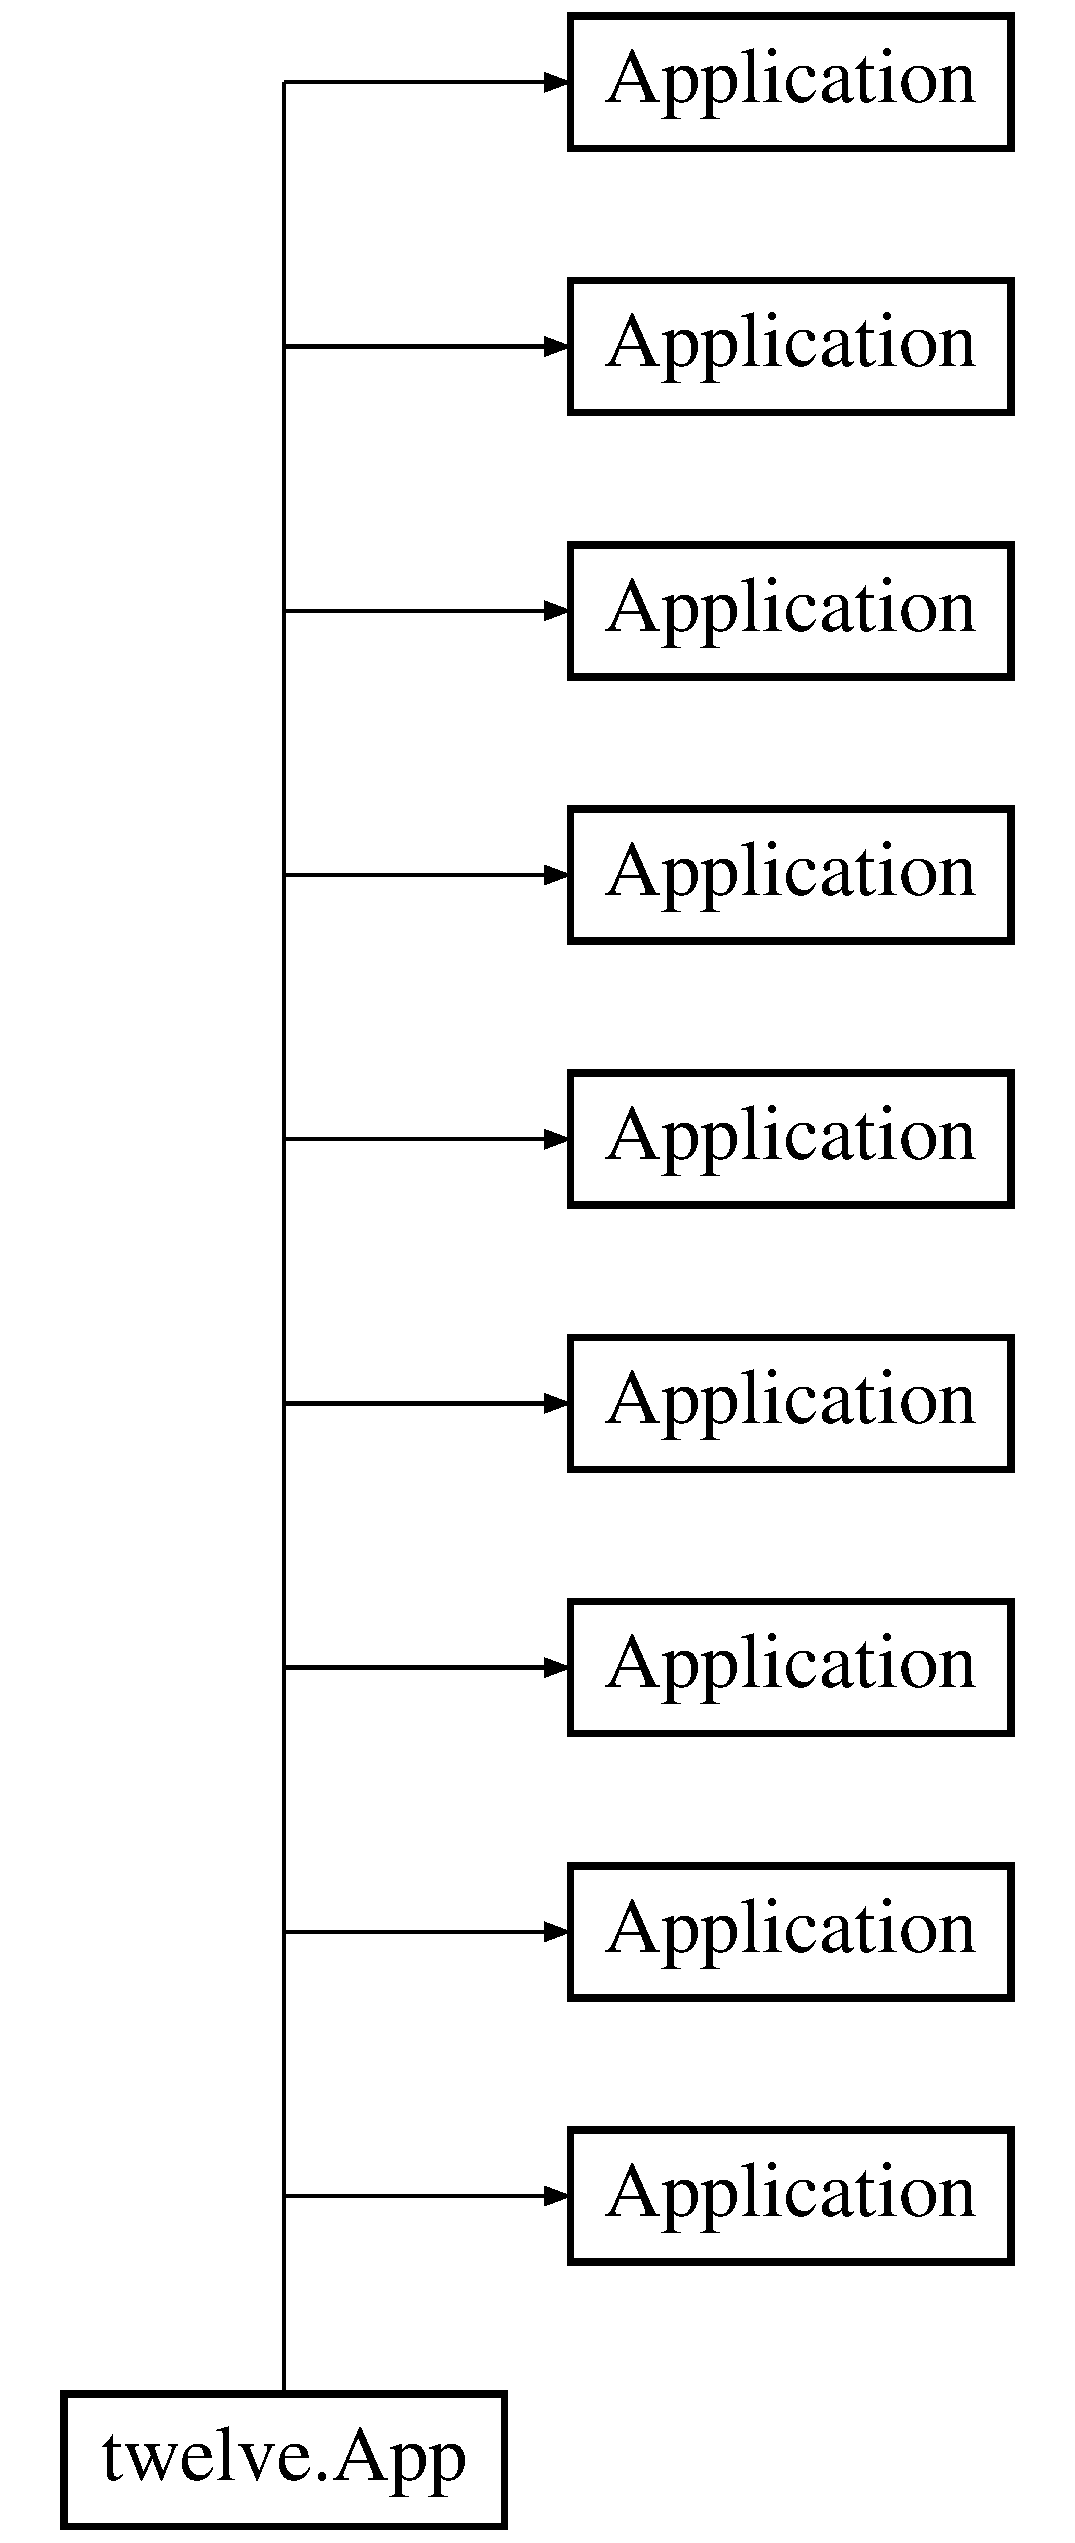
\includegraphics[height=10.000000cm]{classtwelve_1_1_app}
\end{center}
\end{figure}
\subsection*{Public Member Functions}
\begin{DoxyCompactItemize}
\item 
void \hyperlink{classtwelve_1_1_app_ab0d20aed6e986a2ea798b4fc86ae7b10}{Initialize\+Component} ()
\begin{DoxyCompactList}\small\item\em Initialize\+Component \end{DoxyCompactList}\item 
void \hyperlink{classtwelve_1_1_app_ab0d20aed6e986a2ea798b4fc86ae7b10}{Initialize\+Component} ()
\begin{DoxyCompactList}\small\item\em Initialize\+Component \end{DoxyCompactList}\item 
void \hyperlink{classtwelve_1_1_app_ab0d20aed6e986a2ea798b4fc86ae7b10}{Initialize\+Component} ()
\begin{DoxyCompactList}\small\item\em Initialize\+Component \end{DoxyCompactList}\item 
void \hyperlink{classtwelve_1_1_app_ab0d20aed6e986a2ea798b4fc86ae7b10}{Initialize\+Component} ()
\begin{DoxyCompactList}\small\item\em Initialize\+Component \end{DoxyCompactList}\item 
void \hyperlink{classtwelve_1_1_app_ab0d20aed6e986a2ea798b4fc86ae7b10}{Initialize\+Component} ()
\begin{DoxyCompactList}\small\item\em Initialize\+Component \end{DoxyCompactList}\item 
void \hyperlink{classtwelve_1_1_app_ab0d20aed6e986a2ea798b4fc86ae7b10}{Initialize\+Component} ()
\begin{DoxyCompactList}\small\item\em Initialize\+Component \end{DoxyCompactList}\item 
void \hyperlink{classtwelve_1_1_app_ab0d20aed6e986a2ea798b4fc86ae7b10}{Initialize\+Component} ()
\begin{DoxyCompactList}\small\item\em Initialize\+Component \end{DoxyCompactList}\item 
void \hyperlink{classtwelve_1_1_app_ab0d20aed6e986a2ea798b4fc86ae7b10}{Initialize\+Component} ()
\begin{DoxyCompactList}\small\item\em Initialize\+Component \end{DoxyCompactList}\end{DoxyCompactItemize}
\subsection*{Static Public Member Functions}
\begin{DoxyCompactItemize}
\item 
static void \hyperlink{classtwelve_1_1_app_a1450389e259d7675bbb347e9b115328f}{Main} ()
\begin{DoxyCompactList}\small\item\em Application Entry Point. \end{DoxyCompactList}\item 
static void \hyperlink{classtwelve_1_1_app_a1450389e259d7675bbb347e9b115328f}{Main} ()
\begin{DoxyCompactList}\small\item\em Application Entry Point. \end{DoxyCompactList}\item 
static void \hyperlink{classtwelve_1_1_app_a1450389e259d7675bbb347e9b115328f}{Main} ()
\begin{DoxyCompactList}\small\item\em Application Entry Point. \end{DoxyCompactList}\item 
static void \hyperlink{classtwelve_1_1_app_a1450389e259d7675bbb347e9b115328f}{Main} ()
\begin{DoxyCompactList}\small\item\em Application Entry Point. \end{DoxyCompactList}\item 
static void \hyperlink{classtwelve_1_1_app_a1450389e259d7675bbb347e9b115328f}{Main} ()
\begin{DoxyCompactList}\small\item\em Application Entry Point. \end{DoxyCompactList}\item 
static void \hyperlink{classtwelve_1_1_app_a1450389e259d7675bbb347e9b115328f}{Main} ()
\begin{DoxyCompactList}\small\item\em Application Entry Point. \end{DoxyCompactList}\item 
static void \hyperlink{classtwelve_1_1_app_a1450389e259d7675bbb347e9b115328f}{Main} ()
\begin{DoxyCompactList}\small\item\em Application Entry Point. \end{DoxyCompactList}\item 
static void \hyperlink{classtwelve_1_1_app_a1450389e259d7675bbb347e9b115328f}{Main} ()
\begin{DoxyCompactList}\small\item\em Application Entry Point. \end{DoxyCompactList}\end{DoxyCompactItemize}


\subsection{Detailed Description}
Логика взаимодействия для App.\+xaml 

\hyperlink{classtwelve_1_1_app}{App} 

\subsection{Member Function Documentation}
\hypertarget{classtwelve_1_1_app_ab0d20aed6e986a2ea798b4fc86ae7b10}{}\index{twelve\+::\+App@{twelve\+::\+App}!Initialize\+Component@{Initialize\+Component}}
\index{Initialize\+Component@{Initialize\+Component}!twelve\+::\+App@{twelve\+::\+App}}
\subsubsection[{Initialize\+Component}]{\setlength{\rightskip}{0pt plus 5cm}void twelve.\+App.\+Initialize\+Component (
\begin{DoxyParamCaption}
{}
\end{DoxyParamCaption}
)}\label{classtwelve_1_1_app_ab0d20aed6e986a2ea798b4fc86ae7b10}


Initialize\+Component 

\hypertarget{classtwelve_1_1_app_ab0d20aed6e986a2ea798b4fc86ae7b10}{}\index{twelve\+::\+App@{twelve\+::\+App}!Initialize\+Component@{Initialize\+Component}}
\index{Initialize\+Component@{Initialize\+Component}!twelve\+::\+App@{twelve\+::\+App}}
\subsubsection[{Initialize\+Component}]{\setlength{\rightskip}{0pt plus 5cm}void twelve.\+App.\+Initialize\+Component (
\begin{DoxyParamCaption}
{}
\end{DoxyParamCaption}
)}\label{classtwelve_1_1_app_ab0d20aed6e986a2ea798b4fc86ae7b10}


Initialize\+Component 

\hypertarget{classtwelve_1_1_app_ab0d20aed6e986a2ea798b4fc86ae7b10}{}\index{twelve\+::\+App@{twelve\+::\+App}!Initialize\+Component@{Initialize\+Component}}
\index{Initialize\+Component@{Initialize\+Component}!twelve\+::\+App@{twelve\+::\+App}}
\subsubsection[{Initialize\+Component}]{\setlength{\rightskip}{0pt plus 5cm}void twelve.\+App.\+Initialize\+Component (
\begin{DoxyParamCaption}
{}
\end{DoxyParamCaption}
)}\label{classtwelve_1_1_app_ab0d20aed6e986a2ea798b4fc86ae7b10}


Initialize\+Component 

\hypertarget{classtwelve_1_1_app_ab0d20aed6e986a2ea798b4fc86ae7b10}{}\index{twelve\+::\+App@{twelve\+::\+App}!Initialize\+Component@{Initialize\+Component}}
\index{Initialize\+Component@{Initialize\+Component}!twelve\+::\+App@{twelve\+::\+App}}
\subsubsection[{Initialize\+Component}]{\setlength{\rightskip}{0pt plus 5cm}void twelve.\+App.\+Initialize\+Component (
\begin{DoxyParamCaption}
{}
\end{DoxyParamCaption}
)}\label{classtwelve_1_1_app_ab0d20aed6e986a2ea798b4fc86ae7b10}


Initialize\+Component 

\hypertarget{classtwelve_1_1_app_ab0d20aed6e986a2ea798b4fc86ae7b10}{}\index{twelve\+::\+App@{twelve\+::\+App}!Initialize\+Component@{Initialize\+Component}}
\index{Initialize\+Component@{Initialize\+Component}!twelve\+::\+App@{twelve\+::\+App}}
\subsubsection[{Initialize\+Component}]{\setlength{\rightskip}{0pt plus 5cm}void twelve.\+App.\+Initialize\+Component (
\begin{DoxyParamCaption}
{}
\end{DoxyParamCaption}
)}\label{classtwelve_1_1_app_ab0d20aed6e986a2ea798b4fc86ae7b10}


Initialize\+Component 

\hypertarget{classtwelve_1_1_app_ab0d20aed6e986a2ea798b4fc86ae7b10}{}\index{twelve\+::\+App@{twelve\+::\+App}!Initialize\+Component@{Initialize\+Component}}
\index{Initialize\+Component@{Initialize\+Component}!twelve\+::\+App@{twelve\+::\+App}}
\subsubsection[{Initialize\+Component}]{\setlength{\rightskip}{0pt plus 5cm}void twelve.\+App.\+Initialize\+Component (
\begin{DoxyParamCaption}
{}
\end{DoxyParamCaption}
)}\label{classtwelve_1_1_app_ab0d20aed6e986a2ea798b4fc86ae7b10}


Initialize\+Component 

\hypertarget{classtwelve_1_1_app_ab0d20aed6e986a2ea798b4fc86ae7b10}{}\index{twelve\+::\+App@{twelve\+::\+App}!Initialize\+Component@{Initialize\+Component}}
\index{Initialize\+Component@{Initialize\+Component}!twelve\+::\+App@{twelve\+::\+App}}
\subsubsection[{Initialize\+Component}]{\setlength{\rightskip}{0pt plus 5cm}void twelve.\+App.\+Initialize\+Component (
\begin{DoxyParamCaption}
{}
\end{DoxyParamCaption}
)}\label{classtwelve_1_1_app_ab0d20aed6e986a2ea798b4fc86ae7b10}


Initialize\+Component 

\hypertarget{classtwelve_1_1_app_ab0d20aed6e986a2ea798b4fc86ae7b10}{}\index{twelve\+::\+App@{twelve\+::\+App}!Initialize\+Component@{Initialize\+Component}}
\index{Initialize\+Component@{Initialize\+Component}!twelve\+::\+App@{twelve\+::\+App}}
\subsubsection[{Initialize\+Component}]{\setlength{\rightskip}{0pt plus 5cm}void twelve.\+App.\+Initialize\+Component (
\begin{DoxyParamCaption}
{}
\end{DoxyParamCaption}
)}\label{classtwelve_1_1_app_ab0d20aed6e986a2ea798b4fc86ae7b10}


Initialize\+Component 

\hypertarget{classtwelve_1_1_app_a1450389e259d7675bbb347e9b115328f}{}\index{twelve\+::\+App@{twelve\+::\+App}!Main@{Main}}
\index{Main@{Main}!twelve\+::\+App@{twelve\+::\+App}}
\subsubsection[{Main}]{\setlength{\rightskip}{0pt plus 5cm}static void twelve.\+App.\+Main (
\begin{DoxyParamCaption}
{}
\end{DoxyParamCaption}
)\hspace{0.3cm}{\ttfamily [static]}}\label{classtwelve_1_1_app_a1450389e259d7675bbb347e9b115328f}


Application Entry Point. 

\hypertarget{classtwelve_1_1_app_a1450389e259d7675bbb347e9b115328f}{}\index{twelve\+::\+App@{twelve\+::\+App}!Main@{Main}}
\index{Main@{Main}!twelve\+::\+App@{twelve\+::\+App}}
\subsubsection[{Main}]{\setlength{\rightskip}{0pt plus 5cm}static void twelve.\+App.\+Main (
\begin{DoxyParamCaption}
{}
\end{DoxyParamCaption}
)\hspace{0.3cm}{\ttfamily [static]}}\label{classtwelve_1_1_app_a1450389e259d7675bbb347e9b115328f}


Application Entry Point. 

\hypertarget{classtwelve_1_1_app_a1450389e259d7675bbb347e9b115328f}{}\index{twelve\+::\+App@{twelve\+::\+App}!Main@{Main}}
\index{Main@{Main}!twelve\+::\+App@{twelve\+::\+App}}
\subsubsection[{Main}]{\setlength{\rightskip}{0pt plus 5cm}static void twelve.\+App.\+Main (
\begin{DoxyParamCaption}
{}
\end{DoxyParamCaption}
)\hspace{0.3cm}{\ttfamily [static]}}\label{classtwelve_1_1_app_a1450389e259d7675bbb347e9b115328f}


Application Entry Point. 

\hypertarget{classtwelve_1_1_app_a1450389e259d7675bbb347e9b115328f}{}\index{twelve\+::\+App@{twelve\+::\+App}!Main@{Main}}
\index{Main@{Main}!twelve\+::\+App@{twelve\+::\+App}}
\subsubsection[{Main}]{\setlength{\rightskip}{0pt plus 5cm}static void twelve.\+App.\+Main (
\begin{DoxyParamCaption}
{}
\end{DoxyParamCaption}
)\hspace{0.3cm}{\ttfamily [static]}}\label{classtwelve_1_1_app_a1450389e259d7675bbb347e9b115328f}


Application Entry Point. 

\hypertarget{classtwelve_1_1_app_a1450389e259d7675bbb347e9b115328f}{}\index{twelve\+::\+App@{twelve\+::\+App}!Main@{Main}}
\index{Main@{Main}!twelve\+::\+App@{twelve\+::\+App}}
\subsubsection[{Main}]{\setlength{\rightskip}{0pt plus 5cm}static void twelve.\+App.\+Main (
\begin{DoxyParamCaption}
{}
\end{DoxyParamCaption}
)\hspace{0.3cm}{\ttfamily [static]}}\label{classtwelve_1_1_app_a1450389e259d7675bbb347e9b115328f}


Application Entry Point. 

\hypertarget{classtwelve_1_1_app_a1450389e259d7675bbb347e9b115328f}{}\index{twelve\+::\+App@{twelve\+::\+App}!Main@{Main}}
\index{Main@{Main}!twelve\+::\+App@{twelve\+::\+App}}
\subsubsection[{Main}]{\setlength{\rightskip}{0pt plus 5cm}static void twelve.\+App.\+Main (
\begin{DoxyParamCaption}
{}
\end{DoxyParamCaption}
)\hspace{0.3cm}{\ttfamily [static]}}\label{classtwelve_1_1_app_a1450389e259d7675bbb347e9b115328f}


Application Entry Point. 

\hypertarget{classtwelve_1_1_app_a1450389e259d7675bbb347e9b115328f}{}\index{twelve\+::\+App@{twelve\+::\+App}!Main@{Main}}
\index{Main@{Main}!twelve\+::\+App@{twelve\+::\+App}}
\subsubsection[{Main}]{\setlength{\rightskip}{0pt plus 5cm}static void twelve.\+App.\+Main (
\begin{DoxyParamCaption}
{}
\end{DoxyParamCaption}
)\hspace{0.3cm}{\ttfamily [static]}}\label{classtwelve_1_1_app_a1450389e259d7675bbb347e9b115328f}


Application Entry Point. 

\hypertarget{classtwelve_1_1_app_a1450389e259d7675bbb347e9b115328f}{}\index{twelve\+::\+App@{twelve\+::\+App}!Main@{Main}}
\index{Main@{Main}!twelve\+::\+App@{twelve\+::\+App}}
\subsubsection[{Main}]{\setlength{\rightskip}{0pt plus 5cm}static void twelve.\+App.\+Main (
\begin{DoxyParamCaption}
{}
\end{DoxyParamCaption}
)\hspace{0.3cm}{\ttfamily [static]}}\label{classtwelve_1_1_app_a1450389e259d7675bbb347e9b115328f}


Application Entry Point. 



The documentation for this class was generated from the following files\+:\begin{DoxyCompactItemize}
\item 
D\+:/\+Git\+Progects/twelve/twelve/App.\+xaml.\+cs\item 
D\+:/\+Git\+Progects/twelve/twelve/obj/\+Debug/App.\+g.\+cs\item 
D\+:/\+Git\+Progects/twelve/twelve/obj/\+Debug/App.\+g.\+i.\+cs\end{DoxyCompactItemize}

\hypertarget{classtwelve_1_1_converter}{}\section{twelve.\+Converter Class Reference}
\label{classtwelve_1_1_converter}\index{twelve.\+Converter@{twelve.\+Converter}}
\subsection*{Public Member Functions}
\begin{DoxyCompactItemize}
\item 
\hyperlink{classtwelve_1_1_converter_a31ab9582580f65284b4bf6e1fcaf60ca}{Converter} (List$<$ double\mbox{[},\mbox{]}$>$ x, int countline)
\begin{DoxyCompactList}\small\item\em конструктор \end{DoxyCompactList}\item 
Point\+Collection \hyperlink{classtwelve_1_1_converter_a409dedc4a6b066fc0436177266741f99}{getter} ()
\begin{DoxyCompactList}\small\item\em для теста возврат одного значения если ок пусктат в цикл \end{DoxyCompactList}\item 
Point \hyperlink{classtwelve_1_1_converter_a3ece4057a593a4f06bc03dca8dde0cd6}{new\+Point} ()
\begin{DoxyCompactList}\small\item\em cлучайная точка 300 300 \end{DoxyCompactList}\end{DoxyCompactItemize}
\subsection*{Properties}
\begin{DoxyCompactItemize}
\item 
\hypertarget{classtwelve_1_1_converter_abf8b77f35313aa45f084523dbd4f3c92}{}List$<$ Point\+Collection $>$ {\bfseries Mainlist}\hspace{0.3cm}{\ttfamily  \mbox{[}get\mbox{]}}\label{classtwelve_1_1_converter_abf8b77f35313aa45f084523dbd4f3c92}

\end{DoxyCompactItemize}


\subsection{Constructor \& Destructor Documentation}
\hypertarget{classtwelve_1_1_converter_a31ab9582580f65284b4bf6e1fcaf60ca}{}\index{twelve\+::\+Converter@{twelve\+::\+Converter}!Converter@{Converter}}
\index{Converter@{Converter}!twelve\+::\+Converter@{twelve\+::\+Converter}}
\subsubsection[{Converter}]{\setlength{\rightskip}{0pt plus 5cm}twelve.\+Converter.\+Converter (
\begin{DoxyParamCaption}
\item[{List$<$ double\mbox{[},\mbox{]}$>$}]{x, }
\item[{int}]{countline}
\end{DoxyParamCaption}
)}\label{classtwelve_1_1_converter_a31ab9582580f65284b4bf6e1fcaf60ca}


конструктор 


\begin{DoxyParams}{Parameters}
{\em x} & все\\
\hline
{\em countline} & количество линий в фигуре потом считать размер сейчас 8\\
\hline
\end{DoxyParams}


\subsection{Member Function Documentation}
\hypertarget{classtwelve_1_1_converter_a409dedc4a6b066fc0436177266741f99}{}\index{twelve\+::\+Converter@{twelve\+::\+Converter}!getter@{getter}}
\index{getter@{getter}!twelve\+::\+Converter@{twelve\+::\+Converter}}
\subsubsection[{getter}]{\setlength{\rightskip}{0pt plus 5cm}Point\+Collection twelve.\+Converter.\+getter (
\begin{DoxyParamCaption}
{}
\end{DoxyParamCaption}
)}\label{classtwelve_1_1_converter_a409dedc4a6b066fc0436177266741f99}


для теста возврат одного значения если ок пусктат в цикл 

\begin{DoxyReturn}{Returns}

\end{DoxyReturn}
\hypertarget{classtwelve_1_1_converter_a3ece4057a593a4f06bc03dca8dde0cd6}{}\index{twelve\+::\+Converter@{twelve\+::\+Converter}!new\+Point@{new\+Point}}
\index{new\+Point@{new\+Point}!twelve\+::\+Converter@{twelve\+::\+Converter}}
\subsubsection[{new\+Point}]{\setlength{\rightskip}{0pt plus 5cm}Point twelve.\+Converter.\+new\+Point (
\begin{DoxyParamCaption}
{}
\end{DoxyParamCaption}
)}\label{classtwelve_1_1_converter_a3ece4057a593a4f06bc03dca8dde0cd6}


cлучайная точка 300 300 

\begin{DoxyReturn}{Returns}
Point
\end{DoxyReturn}


The documentation for this class was generated from the following file\+:\begin{DoxyCompactItemize}
\item 
D\+:/\+Git\+Progects/twelve/twelve/Converter.\+cs\end{DoxyCompactItemize}

\hypertarget{classtwelve_1_1_filler}{}\section{twelve.\+Filler Class Reference}
\label{classtwelve_1_1_filler}\index{twelve.\+Filler@{twelve.\+Filler}}
\subsection*{Public Member Functions}
\begin{DoxyCompactItemize}
\item 
\hypertarget{classtwelve_1_1_filler_a64d6fd1ae798024fed8fa2e7c7eca9b6}{}{\bfseries Filler} (int ran=8)\label{classtwelve_1_1_filler_a64d6fd1ae798024fed8fa2e7c7eca9b6}

\end{DoxyCompactItemize}
\subsection*{Static Public Member Functions}
\begin{DoxyCompactItemize}
\item 
static void \hyperlink{classtwelve_1_1_filler_a8db08b243d23b903b84a3f2491010a74}{initialization} ()
\begin{DoxyCompactList}\small\item\em начальна инициализация \end{DoxyCompactList}\item 
static void \hyperlink{classtwelve_1_1_filler_a6de2c0a965775e0fec23e8b3468b6082}{search} (Object ka)
\begin{DoxyCompactList}\small\item\em рекурсивная функция \end{DoxyCompactList}\end{DoxyCompactItemize}
\subsection*{Static Public Attributes}
\begin{DoxyCompactItemize}
\item 
\hypertarget{classtwelve_1_1_filler_a3f267327cc923a849f4a542313ca0893}{}static object {\bfseries locker} = new object()\label{classtwelve_1_1_filler_a3f267327cc923a849f4a542313ca0893}

\item 
\hypertarget{classtwelve_1_1_filler_ab3029ab0af96dbe172bd21981e2fb07d}{}static int {\bfseries rank}\label{classtwelve_1_1_filler_ab3029ab0af96dbe172bd21981e2fb07d}

\item 
\hypertarget{classtwelve_1_1_filler_af72f433ecc2ddf7ea00b91f30e55dfae}{}static double\mbox{[},\mbox{]} {\bfseries arr\+Figures}\label{classtwelve_1_1_filler_af72f433ecc2ddf7ea00b91f30e55dfae}

\item 
\hypertarget{classtwelve_1_1_filler_a14576da3f40a0022f1b83dbd02bd3ab9}{}static List$<$ \hyperlink{classtwelve_1_1_little_shape2}{Little\+Shape2} $>$ {\bfseries main\+List\+Colection} = new List$<$\hyperlink{classtwelve_1_1_little_shape2}{Little\+Shape2}$>$()\label{classtwelve_1_1_filler_a14576da3f40a0022f1b83dbd02bd3ab9}

\end{DoxyCompactItemize}


\subsection{Member Function Documentation}
\hypertarget{classtwelve_1_1_filler_a8db08b243d23b903b84a3f2491010a74}{}\index{twelve\+::\+Filler@{twelve\+::\+Filler}!initialization@{initialization}}
\index{initialization@{initialization}!twelve\+::\+Filler@{twelve\+::\+Filler}}
\subsubsection[{initialization}]{\setlength{\rightskip}{0pt plus 5cm}static void twelve.\+Filler.\+initialization (
\begin{DoxyParamCaption}
{}
\end{DoxyParamCaption}
)\hspace{0.3cm}{\ttfamily [static]}}\label{classtwelve_1_1_filler_a8db08b243d23b903b84a3f2491010a74}


начальна инициализация 

\hypertarget{classtwelve_1_1_filler_a6de2c0a965775e0fec23e8b3468b6082}{}\index{twelve\+::\+Filler@{twelve\+::\+Filler}!search@{search}}
\index{search@{search}!twelve\+::\+Filler@{twelve\+::\+Filler}}
\subsubsection[{search}]{\setlength{\rightskip}{0pt plus 5cm}static void twelve.\+Filler.\+search (
\begin{DoxyParamCaption}
\item[{Object}]{ka}
\end{DoxyParamCaption}
)\hspace{0.3cm}{\ttfamily [static]}}\label{classtwelve_1_1_filler_a6de2c0a965775e0fec23e8b3468b6082}


рекурсивная функция 


\begin{DoxyParams}{Parameters}
{\em k} & \\
\hline
\end{DoxyParams}
к=3

test\+Colection.\+Add(temp); 

The documentation for this class was generated from the following file\+:\begin{DoxyCompactItemize}
\item 
D\+:/\+Git\+Progects/twelve/twelve/Fille\+X.\+cs\end{DoxyCompactItemize}

\hypertarget{classtwelve_1_1_filler2}{}\section{twelve.\+Filler2 Class Reference}
\label{classtwelve_1_1_filler2}\index{twelve.\+Filler2@{twelve.\+Filler2}}
\subsection*{Public Member Functions}
\begin{DoxyCompactItemize}
\item 
int \hyperlink{classtwelve_1_1_filler2_ad7dc51c22d12b0e10090b1802cbde9bf}{test\+Rect} (int n, int a, int b, int r)
\item 
\hypertarget{classtwelve_1_1_filler2_ab0858c8ddfd502279085fd0515fd97b5}{}List$<$ int $>$ {\bfseries test\+Fun} ()\label{classtwelve_1_1_filler2_ab0858c8ddfd502279085fd0515fd97b5}

\item 
\hyperlink{classtwelve_1_1_filler2_ac695bd950cff1cc72ab7fc3046f28803}{Filler2} ()
\begin{DoxyCompactList}\small\item\em шаг угла для дележки дерева( для начала 10) число кратное 360 \end{DoxyCompactList}\item 
List$<$ List$<$ int $>$ $>$ \hyperlink{classtwelve_1_1_filler2_a724652dc8868719471ec3f2e60a2bee9}{search\+Main} (int num)
\begin{DoxyCompactList}\small\item\em общая сумма углов для фигуры \end{DoxyCompactList}\item 
bool \hyperlink{classtwelve_1_1_filler2_a86df5048936960aa78ed2e572de1f696}{search} (int breakpoint, ref List$<$ int $>$ arr)
\item 
bool \hyperlink{classtwelve_1_1_filler2_a0aa64ee492904c6aed80d5be8c23de27}{check} (ref List$<$ int $>$ arr, int brekpoint)
\begin{DoxyCompactList}\small\item\em проверка на то перенос из последней стопки в первую false если все перенеслось \end{DoxyCompactList}\item 
bool \hyperlink{classtwelve_1_1_filler2_a2a0dbb1938fcc0150edec9fba4a865ca}{search\+D\+E\+M\+O\+R\+E\+C\+U\+R\+S\+I\+O\+N} (int breakpoint, ref List$<$ int $>$ arr)
\item 
void \hyperlink{classtwelve_1_1_filler2_a1bdbb0a7cdeb105e623833d64cdbb23e}{enlarger2} (ref List$<$ int $>$ arr, int to, int from)
\begin{DoxyCompactList}\small\item\em увеличивает или уменьшает определенную переменнуб в массиве работате как счетчик если невозможно увел тогда false \end{DoxyCompactList}\item 
bool \hyperlink{classtwelve_1_1_filler2_aa463aa40ca8c7bb512bee4bb6d55d86a}{enlarger} (ref List$<$ int $>$ arr, int x)
\end{DoxyCompactItemize}
\subsection*{Static Public Member Functions}
\begin{DoxyCompactItemize}
\item 
\hypertarget{classtwelve_1_1_filler2_af6662a9775f23eb2b2587b4161f3be88}{}static int {\bfseries Fact\+R} (int n)\label{classtwelve_1_1_filler2_af6662a9775f23eb2b2587b4161f3be88}

\end{DoxyCompactItemize}
\subsection*{Public Attributes}
\begin{DoxyCompactItemize}
\item 
\hypertarget{classtwelve_1_1_filler2_a761d6f59cf0c6c82be08fa3f0c0c6e1b}{}List$<$ List$<$ int $>$ $>$ {\bfseries result} = new List$<$List$<$int$>$$>$()\label{classtwelve_1_1_filler2_a761d6f59cf0c6c82be08fa3f0c0c6e1b}

\item 
\hypertarget{classtwelve_1_1_filler2_a709cddffb25ca0a1b4c03deeb7dc9bdc}{}int {\bfseries from}\label{classtwelve_1_1_filler2_a709cddffb25ca0a1b4c03deeb7dc9bdc}

\end{DoxyCompactItemize}


\subsection{Constructor \& Destructor Documentation}
\hypertarget{classtwelve_1_1_filler2_ac695bd950cff1cc72ab7fc3046f28803}{}\index{twelve\+::\+Filler2@{twelve\+::\+Filler2}!Filler2@{Filler2}}
\index{Filler2@{Filler2}!twelve\+::\+Filler2@{twelve\+::\+Filler2}}
\subsubsection[{Filler2}]{\setlength{\rightskip}{0pt plus 5cm}twelve.\+Filler2.\+Filler2 (
\begin{DoxyParamCaption}
{}
\end{DoxyParamCaption}
)}\label{classtwelve_1_1_filler2_ac695bd950cff1cc72ab7fc3046f28803}


шаг угла для дележки дерева( для начала 10) число кратное 360 


\begin{DoxyParams}{Parameters}
{\em step} & \\
\hline
\end{DoxyParams}


\subsection{Member Function Documentation}
\hypertarget{classtwelve_1_1_filler2_a0aa64ee492904c6aed80d5be8c23de27}{}\index{twelve\+::\+Filler2@{twelve\+::\+Filler2}!check@{check}}
\index{check@{check}!twelve\+::\+Filler2@{twelve\+::\+Filler2}}
\subsubsection[{check}]{\setlength{\rightskip}{0pt plus 5cm}bool twelve.\+Filler2.\+check (
\begin{DoxyParamCaption}
\item[{ref List$<$ int $>$}]{arr, }
\item[{int}]{brekpoint}
\end{DoxyParamCaption}
)}\label{classtwelve_1_1_filler2_a0aa64ee492904c6aed80d5be8c23de27}


проверка на то перенос из последней стопки в первую false если все перенеслось 


\begin{DoxyParams}{Parameters}
{\em arr} & \\
\hline
{\em brecpoint} & \\
\hline
\end{DoxyParams}
\begin{DoxyReturn}{Returns}
false если все перенеслось
\end{DoxyReturn}
\hypertarget{classtwelve_1_1_filler2_aa463aa40ca8c7bb512bee4bb6d55d86a}{}\index{twelve\+::\+Filler2@{twelve\+::\+Filler2}!enlarger@{enlarger}}
\index{enlarger@{enlarger}!twelve\+::\+Filler2@{twelve\+::\+Filler2}}
\subsubsection[{enlarger}]{\setlength{\rightskip}{0pt plus 5cm}bool twelve.\+Filler2.\+enlarger (
\begin{DoxyParamCaption}
\item[{ref List$<$ int $>$}]{arr, }
\item[{int}]{x}
\end{DoxyParamCaption}
)}\label{classtwelve_1_1_filler2_aa463aa40ca8c7bb512bee4bb6d55d86a}




увеличивает или уменьшает определенную переменнуб в массиве работате как счетчик если невозможно увел тогда false 


\begin{DoxyParams}{Parameters}
{\em arr} & массив\\
\hline
{\em x} & максимальное значение\\
\hline
\end{DoxyParams}
\hypertarget{classtwelve_1_1_filler2_a1bdbb0a7cdeb105e623833d64cdbb23e}{}\index{twelve\+::\+Filler2@{twelve\+::\+Filler2}!enlarger2@{enlarger2}}
\index{enlarger2@{enlarger2}!twelve\+::\+Filler2@{twelve\+::\+Filler2}}
\subsubsection[{enlarger2}]{\setlength{\rightskip}{0pt plus 5cm}void twelve.\+Filler2.\+enlarger2 (
\begin{DoxyParamCaption}
\item[{ref List$<$ int $>$}]{arr, }
\item[{int}]{to, }
\item[{int}]{from}
\end{DoxyParamCaption}
)}\label{classtwelve_1_1_filler2_a1bdbb0a7cdeb105e623833d64cdbb23e}


увеличивает или уменьшает определенную переменнуб в массиве работате как счетчик если невозможно увел тогда false 


\begin{DoxyParams}{Parameters}
{\em arr} & массив\\
\hline
{\em x} & максимальное значение\\
\hline
\end{DoxyParams}
\hypertarget{classtwelve_1_1_filler2_a86df5048936960aa78ed2e572de1f696}{}\index{twelve\+::\+Filler2@{twelve\+::\+Filler2}!search@{search}}
\index{search@{search}!twelve\+::\+Filler2@{twelve\+::\+Filler2}}
\subsubsection[{search}]{\setlength{\rightskip}{0pt plus 5cm}bool twelve.\+Filler2.\+search (
\begin{DoxyParamCaption}
\item[{int}]{breakpoint, }
\item[{ref List$<$ int $>$}]{arr}
\end{DoxyParamCaption}
)}\label{classtwelve_1_1_filler2_a86df5048936960aa78ed2e572de1f696}





\begin{DoxyParams}{Parameters}
{\em breakpoint} & сумма углов минус количество граней для квадрата \mbox{[}360-\/3\mbox{]} \\
\hline
{\em arr} & массив с начальними значениями \mbox{[}1\mbox{]}\mbox{[}1\mbox{]}\mbox{[}1\mbox{]}\mbox{[}360-\/3\mbox{]} для квадрата\\
\hline
\end{DoxyParams}
\begin{DoxyReturn}{Returns}

\end{DoxyReturn}
\hypertarget{classtwelve_1_1_filler2_a2a0dbb1938fcc0150edec9fba4a865ca}{}\index{twelve\+::\+Filler2@{twelve\+::\+Filler2}!search\+D\+E\+M\+O\+R\+E\+C\+U\+R\+S\+I\+O\+N@{search\+D\+E\+M\+O\+R\+E\+C\+U\+R\+S\+I\+O\+N}}
\index{search\+D\+E\+M\+O\+R\+E\+C\+U\+R\+S\+I\+O\+N@{search\+D\+E\+M\+O\+R\+E\+C\+U\+R\+S\+I\+O\+N}!twelve\+::\+Filler2@{twelve\+::\+Filler2}}
\subsubsection[{search\+D\+E\+M\+O\+R\+E\+C\+U\+R\+S\+I\+O\+N}]{\setlength{\rightskip}{0pt plus 5cm}bool twelve.\+Filler2.\+search\+D\+E\+M\+O\+R\+E\+C\+U\+R\+S\+I\+O\+N (
\begin{DoxyParamCaption}
\item[{int}]{breakpoint, }
\item[{ref List$<$ int $>$}]{arr}
\end{DoxyParamCaption}
)}\label{classtwelve_1_1_filler2_a2a0dbb1938fcc0150edec9fba4a865ca}





\begin{DoxyParams}{Parameters}
{\em breakpoint} & сумма углов минус количество граней для квадрата \mbox{[}360-\/3\mbox{]} \\
\hline
{\em arr} & массив с начальними значениями \mbox{[}1\mbox{]}\mbox{[}1\mbox{]}\mbox{[}1\mbox{]}\mbox{[}360-\/3\mbox{]} для квадрата\\
\hline
\end{DoxyParams}
\begin{DoxyReturn}{Returns}

\end{DoxyReturn}
\hypertarget{classtwelve_1_1_filler2_a724652dc8868719471ec3f2e60a2bee9}{}\index{twelve\+::\+Filler2@{twelve\+::\+Filler2}!search\+Main@{search\+Main}}
\index{search\+Main@{search\+Main}!twelve\+::\+Filler2@{twelve\+::\+Filler2}}
\subsubsection[{search\+Main}]{\setlength{\rightskip}{0pt plus 5cm}List$<$List$<$int$>$ $>$ twelve.\+Filler2.\+search\+Main (
\begin{DoxyParamCaption}
\item[{int}]{num}
\end{DoxyParamCaption}
)}\label{classtwelve_1_1_filler2_a724652dc8868719471ec3f2e60a2bee9}


общая сумма углов для фигуры 

\href{https://ru.wikipedia.org/wiki/%D0%A2%D0%B5%D0%BE%D1%80%D0%B5%D0%BC%D0%B0_%D0%BE_%D1%81%D1%83%D0%BC%D0%BC%D0%B5_%D1%83%D0%B3%D0%BB%D0%BE%D0%B2_%D0%BC%D0%BD%D0%BE%D0%B3%D0%BE%D1%83%D0%B3%D0%BE%D0%BB%D1%8C%D0%BD%D0%B8%D0%BA%D0%B0}{\tt https\+://ru.\+wikipedia.\+org/wiki/\%\+D0\%\+A2\%\+D0\%\+B5\%\+D0\%\+B\+E\%\+D1\%80\%\+D0\%\+B5\%\+D0\%\+B\+C\%\+D0\%\+B0\+\_\+\%\+D0\%\+B\+E\+\_\+\%\+D1\%81\%\+D1\%83\%\+D0\%\+B\+C\%\+D0\%\+B\+C\%\+D0\%\+B5\+\_\+\%\+D1\%83\%\+D0\%\+B3\%\+D0\%\+B\+B\%\+D0\%\+B\+E\%\+D0\%\+B2\+\_\+\%\+D0\%\+B\+C\%\+D0\%\+B\+D\%\+D0\%\+B\+E\%\+D0\%\+B3\%\+D0\%\+B\+E\%\+D1\%83\%\+D0\%\+B3\%\+D0\%\+B\+E\%\+D0\%\+B\+B\%\+D1\%8\+C\%\+D0\%\+B\+D\%\+D0\%\+B8\%\+D0\%\+B\+A\%\+D0\%\+B0} 


\begin{DoxyParams}{Parameters}
{\em x} & количество дуг число не менне 4 !!!\\
\hline
\end{DoxyParams}
\begin{DoxyReturn}{Returns}
общая сума
\end{DoxyReturn}
\hypertarget{classtwelve_1_1_filler2_ad7dc51c22d12b0e10090b1802cbde9bf}{}\index{twelve\+::\+Filler2@{twelve\+::\+Filler2}!test\+Rect@{test\+Rect}}
\index{test\+Rect@{test\+Rect}!twelve\+::\+Filler2@{twelve\+::\+Filler2}}
\subsubsection[{test\+Rect}]{\setlength{\rightskip}{0pt plus 5cm}int twelve.\+Filler2.\+test\+Rect (
\begin{DoxyParamCaption}
\item[{int}]{n, }
\item[{int}]{a, }
\item[{int}]{b, }
\item[{int}]{r}
\end{DoxyParamCaption}
)}\label{classtwelve_1_1_filler2_ad7dc51c22d12b0e10090b1802cbde9bf}
найти те числа какие сумма каких равна даному числу 

The documentation for this class was generated from the following file\+:\begin{DoxyCompactItemize}
\item 
D\+:/\+Git\+Progects/twelve/twelve/Filler2.\+cs\end{DoxyCompactItemize}

\hypertarget{classtwelve_1_1_filler3}{}\section{twelve.\+Filler3 Class Reference}
\label{classtwelve_1_1_filler3}\index{twelve.\+Filler3@{twelve.\+Filler3}}
\subsection*{Public Member Functions}
\begin{DoxyCompactItemize}
\item 
\hypertarget{classtwelve_1_1_filler3_af4f4768c36421a10016b22b440ba0c61}{}bool {\bfseries search} ()\label{classtwelve_1_1_filler3_af4f4768c36421a10016b22b440ba0c61}

\item 
\hypertarget{classtwelve_1_1_filler3_a11430ce8d4476fda83c92665ae9672a1}{}Point {\bfseries new\+Point} (ref List$<$ Point $>$ arr, double degree)\label{classtwelve_1_1_filler3_a11430ce8d4476fda83c92665ae9672a1}

\item 
\hypertarget{classtwelve_1_1_filler3_a379abecc1e27ee2162e55c5aa006ceff}{}Point {\bfseries new\+Point} (double degree)\label{classtwelve_1_1_filler3_a379abecc1e27ee2162e55c5aa006ceff}

\item 
\hypertarget{classtwelve_1_1_filler3_a9122e4bbd751fc1220e54f3b03c3dfd7}{}int {\bfseries quartern} ()\label{classtwelve_1_1_filler3_a9122e4bbd751fc1220e54f3b03c3dfd7}

\item 
\hyperlink{classtwelve_1_1_filler3_a7576e5701848fcf85d1d45e87f0976b3}{Filler3} (int rank=4, double angle=90)
\end{DoxyCompactItemize}
\subsection*{Public Attributes}
\begin{DoxyCompactItemize}
\item 
\hypertarget{classtwelve_1_1_filler3_a53765f88bd16daa9de14cf43ac5f51ce}{}List$<$ List$<$ Point $>$ $>$ {\bfseries main\+Colections} = new List$<$List$<$Point$>$$>$()\label{classtwelve_1_1_filler3_a53765f88bd16daa9de14cf43ac5f51ce}

\item 
\hypertarget{classtwelve_1_1_filler3_a034b1e0e5f4c90387489177b3876c6da}{}List$<$ Point $>$ {\bfseries main\+Point\+List} = new List$<$Point$>$()\label{classtwelve_1_1_filler3_a034b1e0e5f4c90387489177b3876c6da}

\item 
\hypertarget{classtwelve_1_1_filler3_abbc656d410485898fa9a574bc8119ef4}{}List$<$ Point $>$ {\bfseries redy\+Points} = new List$<$Point$>$()\label{classtwelve_1_1_filler3_abbc656d410485898fa9a574bc8119ef4}

\item 
\hypertarget{classtwelve_1_1_filler3_a2d4756240736dff04d60bc687ea7311c}{}List$<$ double $>$ {\bfseries arr\+Degree} = new List$<$double$>$ ()\label{classtwelve_1_1_filler3_a2d4756240736dff04d60bc687ea7311c}

\item 
\hypertarget{classtwelve_1_1_filler3_a06d88298e6427d437fca742036f188cf}{}List$<$ double $>$ {\bfseries test} = new List$<$double$>$ \{0, 30, 90,210\}\label{classtwelve_1_1_filler3_a06d88298e6427d437fca742036f188cf}

\end{DoxyCompactItemize}


\subsection{Constructor \& Destructor Documentation}
\hypertarget{classtwelve_1_1_filler3_a7576e5701848fcf85d1d45e87f0976b3}{}\index{twelve\+::\+Filler3@{twelve\+::\+Filler3}!Filler3@{Filler3}}
\index{Filler3@{Filler3}!twelve\+::\+Filler3@{twelve\+::\+Filler3}}
\subsubsection[{Filler3}]{\setlength{\rightskip}{0pt plus 5cm}twelve.\+Filler3.\+Filler3 (
\begin{DoxyParamCaption}
\item[{int}]{rank = {\ttfamily 4}, }
\item[{double}]{angle = {\ttfamily 90}}
\end{DoxyParamCaption}
)}\label{classtwelve_1_1_filler3_a7576e5701848fcf85d1d45e87f0976b3}





\begin{DoxyParams}{Parameters}
{\em rank} & количество поколений сейчас 4 для квадрата\\
\hline
{\em angle} & статичный градус сейчас 90\\
\hline
\end{DoxyParams}


The documentation for this class was generated from the following file\+:\begin{DoxyCompactItemize}
\item 
D\+:/\+Git\+Progects/twelve/twelve/Filler3.\+cs\end{DoxyCompactItemize}

\hypertarget{classtwelve_1_1_filler4}{}\section{twelve.\+Filler4 Class Reference}
\label{classtwelve_1_1_filler4}\index{twelve.\+Filler4@{twelve.\+Filler4}}
\subsection*{Public Member Functions}
\begin{DoxyCompactItemize}
\item 
\hypertarget{classtwelve_1_1_filler4_ae90c551fb31a72f754c10abb9e2085e8}{}void {\bfseries test} ()\label{classtwelve_1_1_filler4_ae90c551fb31a72f754c10abb9e2085e8}

\item 
void \hyperlink{classtwelve_1_1_filler4_afdd6ca004450f41ac14033e53480d4b3}{shift\+Array} (ref Point\mbox{[}$\,$\mbox{]} arr, Point p)
\begin{DoxyCompactList}\small\item\em смещение все точек на -\/х и -\/у \end{DoxyCompactList}\item 
\hypertarget{classtwelve_1_1_filler4_aff950ffda0ccfb0fa884b19be68c67ce}{}Point {\bfseries new\+Point} (double degree)\label{classtwelve_1_1_filler4_aff950ffda0ccfb0fa884b19be68c67ce}

\end{DoxyCompactItemize}


\subsection{Member Function Documentation}
\hypertarget{classtwelve_1_1_filler4_afdd6ca004450f41ac14033e53480d4b3}{}\index{twelve\+::\+Filler4@{twelve\+::\+Filler4}!shift\+Array@{shift\+Array}}
\index{shift\+Array@{shift\+Array}!twelve\+::\+Filler4@{twelve\+::\+Filler4}}
\subsubsection[{shift\+Array}]{\setlength{\rightskip}{0pt plus 5cm}void twelve.\+Filler4.\+shift\+Array (
\begin{DoxyParamCaption}
\item[{ref Point\mbox{[}$\,$\mbox{]}}]{arr, }
\item[{Point}]{p}
\end{DoxyParamCaption}
)}\label{classtwelve_1_1_filler4_afdd6ca004450f41ac14033e53480d4b3}


смещение все точек на -\/х и -\/у 


\begin{DoxyParams}{Parameters}
{\em arr} & \\
\hline
{\em p} & \\
\hline
\end{DoxyParams}


The documentation for this class was generated from the following file\+:\begin{DoxyCompactItemize}
\item 
D\+:/\+Git\+Progects/twelve/twelve/Filler4.\+cs\end{DoxyCompactItemize}

\hypertarget{classtwelve_1_1_filler5}{}\section{twelve.\+Filler5 Class Reference}
\label{classtwelve_1_1_filler5}\index{twelve.\+Filler5@{twelve.\+Filler5}}
\subsection*{Public Member Functions}
\begin{DoxyCompactItemize}
\item 
void \hyperlink{classtwelve_1_1_filler5_a05e5629690a63eec09ea71df3373a0c3}{shift\+Array} (ref Point\mbox{[}$\,$\mbox{]} arr, Point p)
\begin{DoxyCompactList}\small\item\em смещение все точек на -\/х и -\/у \end{DoxyCompactList}\item 
void \hyperlink{classtwelve_1_1_filler5_a0c70a6f5d57489a287b9f33e47cc110f}{shift\+Array2} (ref Point\mbox{[}$\,$\mbox{]} arr, Point p)
\begin{DoxyCompactList}\small\item\em смещение все точек на -\/х и -\/у \end{DoxyCompactList}\item 
\hypertarget{classtwelve_1_1_filler5_a8a967b46734cba6e74a0f0bf26734318}{}void {\bfseries start} ()\label{classtwelve_1_1_filler5_a8a967b46734cba6e74a0f0bf26734318}

\item 
\hypertarget{classtwelve_1_1_filler5_ad719bd5b70ec6697c71823a5e3fcd102}{}bool {\bfseries search} ()\label{classtwelve_1_1_filler5_ad719bd5b70ec6697c71823a5e3fcd102}

\item 
\hypertarget{classtwelve_1_1_filler5_ad7e4993138b35a7188160c97a62767ea}{}Point {\bfseries new\+Point} (double degree)\label{classtwelve_1_1_filler5_ad7e4993138b35a7188160c97a62767ea}

\item 
\hypertarget{classtwelve_1_1_filler5_ab20c7d27b839ac157f19b38b769d883a}{}{\bfseries Filler5} (Canvas can, int rank=5, double deg=30)\label{classtwelve_1_1_filler5_ab20c7d27b839ac157f19b38b769d883a}

\item 
\hypertarget{classtwelve_1_1_filler5_ac358653a36f3c87a247576f76f3ed776}{}void {\bfseries draw\+Of\+Index} (int index)\label{classtwelve_1_1_filler5_ac358653a36f3c87a247576f76f3ed776}

\item 
\hypertarget{classtwelve_1_1_filler5_a1d1af46cd86664d98faa5877101cbabd}{}void {\bfseries draw} ()\label{classtwelve_1_1_filler5_a1d1af46cd86664d98faa5877101cbabd}

\item 
\hypertarget{classtwelve_1_1_filler5_aa6e41f5cabb22941934044df16efad3e}{}void {\bfseries scale\+Curent\+Figure2} (ref Point\mbox{[}$\,$\mbox{]} p)\label{classtwelve_1_1_filler5_aa6e41f5cabb22941934044df16efad3e}

\item 
\hypertarget{classtwelve_1_1_filler5_a092e3bb1a23afdeddfc5166172447559}{}void {\bfseries scale\+Curent\+Figure} ()\label{classtwelve_1_1_filler5_a092e3bb1a23afdeddfc5166172447559}

\item 
\hypertarget{classtwelve_1_1_filler5_a9b4e7d6b572af8aed3a0c88edda737a7}{}void {\bfseries Stream\+Geometry\+Triangle\+Example} (List$<$ System.\+Windows.\+Point $>$ arr\+Points)\label{classtwelve_1_1_filler5_a9b4e7d6b572af8aed3a0c88edda737a7}

\end{DoxyCompactItemize}
\subsection*{Public Attributes}
\begin{DoxyCompactItemize}
\item 
\hypertarget{classtwelve_1_1_filler5_a53d8833afa3b9a40f041adb5719f42d4}{}List$<$ Point\mbox{[}$\,$\mbox{]}$>$ {\bfseries main\+Colections} = new List$<$Point\mbox{[}$\,$\mbox{]}$>$()\label{classtwelve_1_1_filler5_a53d8833afa3b9a40f041adb5719f42d4}

\end{DoxyCompactItemize}


\subsection{Member Function Documentation}
\hypertarget{classtwelve_1_1_filler5_a05e5629690a63eec09ea71df3373a0c3}{}\index{twelve\+::\+Filler5@{twelve\+::\+Filler5}!shift\+Array@{shift\+Array}}
\index{shift\+Array@{shift\+Array}!twelve\+::\+Filler5@{twelve\+::\+Filler5}}
\subsubsection[{shift\+Array}]{\setlength{\rightskip}{0pt plus 5cm}void twelve.\+Filler5.\+shift\+Array (
\begin{DoxyParamCaption}
\item[{ref Point\mbox{[}$\,$\mbox{]}}]{arr, }
\item[{Point}]{p}
\end{DoxyParamCaption}
)}\label{classtwelve_1_1_filler5_a05e5629690a63eec09ea71df3373a0c3}


смещение все точек на -\/х и -\/у 


\begin{DoxyParams}{Parameters}
{\em arr} & \\
\hline
{\em p} & \\
\hline
\end{DoxyParams}
\hypertarget{classtwelve_1_1_filler5_a0c70a6f5d57489a287b9f33e47cc110f}{}\index{twelve\+::\+Filler5@{twelve\+::\+Filler5}!shift\+Array2@{shift\+Array2}}
\index{shift\+Array2@{shift\+Array2}!twelve\+::\+Filler5@{twelve\+::\+Filler5}}
\subsubsection[{shift\+Array2}]{\setlength{\rightskip}{0pt plus 5cm}void twelve.\+Filler5.\+shift\+Array2 (
\begin{DoxyParamCaption}
\item[{ref Point\mbox{[}$\,$\mbox{]}}]{arr, }
\item[{Point}]{p}
\end{DoxyParamCaption}
)}\label{classtwelve_1_1_filler5_a0c70a6f5d57489a287b9f33e47cc110f}


смещение все точек на -\/х и -\/у 


\begin{DoxyParams}{Parameters}
{\em arr} & \\
\hline
{\em p} & \\
\hline
\end{DoxyParams}


The documentation for this class was generated from the following file\+:\begin{DoxyCompactItemize}
\item 
D\+:/\+Git\+Progects/twelve/twelve/Filler5.\+cs\end{DoxyCompactItemize}

\hypertarget{classtwelve_1_1_filler6}{}\section{twelve.\+Filler6 Class Reference}
\label{classtwelve_1_1_filler6}\index{twelve.\+Filler6@{twelve.\+Filler6}}
\subsection*{Public Member Functions}
\begin{DoxyCompactItemize}
\item 
\hypertarget{classtwelve_1_1_filler6_a2a590a9047b60772c8449842ce56295b}{}void {\bfseries start} ()\label{classtwelve_1_1_filler6_a2a590a9047b60772c8449842ce56295b}

\item 
\hypertarget{classtwelve_1_1_filler6_a7b0be121b51b1b8f6a51216373409917}{}bool {\bfseries alif} (double degree)\label{classtwelve_1_1_filler6_a7b0be121b51b1b8f6a51216373409917}

\item 
\hypertarget{classtwelve_1_1_filler6_a9466bf337125eb593ebdd9916fc81798}{}Point {\bfseries search} (ref Point\mbox{[}$\,$\mbox{]} arr, Point p, double angle, int level)\label{classtwelve_1_1_filler6_a9466bf337125eb593ebdd9916fc81798}

\item 
bool \hyperlink{classtwelve_1_1_filler6_a102142ff7777081638239014909ac71e}{first\+Check} (Point\mbox{[}$\,$\mbox{]} main\+Poins2, Point p)
\begin{DoxyCompactList}\small\item\em первая проверка в самом низу на \end{DoxyCompactList}\item 
Point \hyperlink{classtwelve_1_1_filler6_a9aec4e377da21a969f4ac1d8c2ef9d39}{new\+Point} (double degree)
\begin{DoxyCompactList}\small\item\em новая точка \end{DoxyCompactList}\item 
void \hyperlink{classtwelve_1_1_filler6_a1140cb98c5a30ff7d6f99fc42c7fe253}{shift\+Array} (ref Point\mbox{[}$\,$\mbox{]} arr, Point p)
\begin{DoxyCompactList}\small\item\em смещение все точек на -\/х и -\/у \end{DoxyCompactList}\item 
\hypertarget{classtwelve_1_1_filler6_a1d41e6f83ef0bc073fa36d605528f3c1}{}void {\bfseries shift\+List} (ref List$<$ Point $>$ arr, Point p)\label{classtwelve_1_1_filler6_a1d41e6f83ef0bc073fa36d605528f3c1}

\item 
\hypertarget{classtwelve_1_1_filler6_a0c312517f962aa708a0662470476b0d5}{}void {\bfseries draw\+Of\+Index} (int index)\label{classtwelve_1_1_filler6_a0c312517f962aa708a0662470476b0d5}

\item 
\hypertarget{classtwelve_1_1_filler6_af0f697fe0039b2f9d1886e7798621503}{}void {\bfseries draw} ()\label{classtwelve_1_1_filler6_af0f697fe0039b2f9d1886e7798621503}

\item 
\hypertarget{classtwelve_1_1_filler6_a4cac0fa6ebf8c9ab69e812d4c0842a5c}{}void {\bfseries scale\+Curent\+Figure2} (ref Point\mbox{[}$\,$\mbox{]} p)\label{classtwelve_1_1_filler6_a4cac0fa6ebf8c9ab69e812d4c0842a5c}

\item 
\hypertarget{classtwelve_1_1_filler6_a84243055aa0412190507caefc70f10b2}{}void {\bfseries scale\+Curent\+Figure} ()\label{classtwelve_1_1_filler6_a84243055aa0412190507caefc70f10b2}

\item 
\hypertarget{classtwelve_1_1_filler6_a8189c4900c689a1bdfb00d9d89ebabb1}{}void {\bfseries Stream\+Geometry\+Triangle\+Example} (List$<$ System.\+Windows.\+Point $>$ arr\+Points)\label{classtwelve_1_1_filler6_a8189c4900c689a1bdfb00d9d89ebabb1}

\item 
\hyperlink{classtwelve_1_1_filler6_afb5bcc7ec2b0f39501fe2442a34ae0ce}{Filler6} (Canvas can, int rank=4, double deg=30)
\end{DoxyCompactItemize}
\subsection*{Public Attributes}
\begin{DoxyCompactItemize}
\item 
\hypertarget{classtwelve_1_1_filler6_a17bc3075b5dbbe55f0e0275912043bcc}{}List$<$ Point\mbox{[}$\,$\mbox{]}$>$ {\bfseries main\+Colections} = new List$<$Point\mbox{[}$\,$\mbox{]}$>$()\label{classtwelve_1_1_filler6_a17bc3075b5dbbe55f0e0275912043bcc}

\item 
\hypertarget{classtwelve_1_1_filler6_a4bc8a80db9edc1c66efd79b1f30f785c}{}List$<$ Point $>$ {\bfseries temp\+Popint\+List} = new List$<$Point$>$()\label{classtwelve_1_1_filler6_a4bc8a80db9edc1c66efd79b1f30f785c}

\item 
\hypertarget{classtwelve_1_1_filler6_a813212083a003c7229ac49d9da67a92b}{}List$<$ Point $>$ {\bfseries colect\+Point\+For\+Zero} = new List$<$Point$>$()\label{classtwelve_1_1_filler6_a813212083a003c7229ac49d9da67a92b}

\end{DoxyCompactItemize}


\subsection{Constructor \& Destructor Documentation}
\hypertarget{classtwelve_1_1_filler6_afb5bcc7ec2b0f39501fe2442a34ae0ce}{}\index{twelve\+::\+Filler6@{twelve\+::\+Filler6}!Filler6@{Filler6}}
\index{Filler6@{Filler6}!twelve\+::\+Filler6@{twelve\+::\+Filler6}}
\subsubsection[{Filler6}]{\setlength{\rightskip}{0pt plus 5cm}twelve.\+Filler6.\+Filler6 (
\begin{DoxyParamCaption}
\item[{Canvas}]{can, }
\item[{int}]{rank = {\ttfamily 4}, }
\item[{double}]{deg = {\ttfamily 30}}
\end{DoxyParamCaption}
)}\label{classtwelve_1_1_filler6_afb5bcc7ec2b0f39501fe2442a34ae0ce}





\begin{DoxyParams}{Parameters}
{\em can} & \\
\hline
{\em rank} & для квадрата 4 точка\\
\hline
{\em deg} & \\
\hline
\end{DoxyParams}


\subsection{Member Function Documentation}
\hypertarget{classtwelve_1_1_filler6_a102142ff7777081638239014909ac71e}{}\index{twelve\+::\+Filler6@{twelve\+::\+Filler6}!first\+Check@{first\+Check}}
\index{first\+Check@{first\+Check}!twelve\+::\+Filler6@{twelve\+::\+Filler6}}
\subsubsection[{first\+Check}]{\setlength{\rightskip}{0pt plus 5cm}bool twelve.\+Filler6.\+first\+Check (
\begin{DoxyParamCaption}
\item[{Point\mbox{[}$\,$\mbox{]}}]{main\+Poins2, }
\item[{Point}]{p}
\end{DoxyParamCaption}
)}\label{classtwelve_1_1_filler6_a102142ff7777081638239014909ac71e}


первая проверка в самом низу на 

\begin{DoxyReturn}{Returns}
+ it\textquotesingle{}s ok point is
\end{DoxyReturn}
\hypertarget{classtwelve_1_1_filler6_a9aec4e377da21a969f4ac1d8c2ef9d39}{}\index{twelve\+::\+Filler6@{twelve\+::\+Filler6}!new\+Point@{new\+Point}}
\index{new\+Point@{new\+Point}!twelve\+::\+Filler6@{twelve\+::\+Filler6}}
\subsubsection[{new\+Point}]{\setlength{\rightskip}{0pt plus 5cm}Point twelve.\+Filler6.\+new\+Point (
\begin{DoxyParamCaption}
\item[{double}]{degree}
\end{DoxyParamCaption}
)}\label{classtwelve_1_1_filler6_a9aec4e377da21a969f4ac1d8c2ef9d39}


новая точка 


\begin{DoxyParams}{Parameters}
{\em degree} & \\
\hline
\end{DoxyParams}
\begin{DoxyReturn}{Returns}

\end{DoxyReturn}
\hypertarget{classtwelve_1_1_filler6_a1140cb98c5a30ff7d6f99fc42c7fe253}{}\index{twelve\+::\+Filler6@{twelve\+::\+Filler6}!shift\+Array@{shift\+Array}}
\index{shift\+Array@{shift\+Array}!twelve\+::\+Filler6@{twelve\+::\+Filler6}}
\subsubsection[{shift\+Array}]{\setlength{\rightskip}{0pt plus 5cm}void twelve.\+Filler6.\+shift\+Array (
\begin{DoxyParamCaption}
\item[{ref Point\mbox{[}$\,$\mbox{]}}]{arr, }
\item[{Point}]{p}
\end{DoxyParamCaption}
)}\label{classtwelve_1_1_filler6_a1140cb98c5a30ff7d6f99fc42c7fe253}


смещение все точек на -\/х и -\/у 


\begin{DoxyParams}{Parameters}
{\em arr} & \\
\hline
{\em p} & \\
\hline
\end{DoxyParams}


The documentation for this class was generated from the following file\+:\begin{DoxyCompactItemize}
\item 
D\+:/\+Git\+Progects/twelve/twelve/Filler6.\+cs\end{DoxyCompactItemize}

\hypertarget{classtwelve_1_1_filler7}{}\section{twelve.\+Filler7 Class Reference}
\label{classtwelve_1_1_filler7}\index{twelve.\+Filler7@{twelve.\+Filler7}}
\subsection*{Public Member Functions}
\begin{DoxyCompactItemize}
\item 
\hypertarget{classtwelve_1_1_filler7_a5f9cb0b5b59c1c4a4e51da34b5caafde}{}void {\bfseries start} ()\label{classtwelve_1_1_filler7_a5f9cb0b5b59c1c4a4e51da34b5caafde}

\item 
Point \hyperlink{classtwelve_1_1_filler7_a6b358aba8dcf1dc4e05e276c603d9f38}{new\+Point} (double degree)
\begin{DoxyCompactList}\small\item\em новая точка \end{DoxyCompactList}\end{DoxyCompactItemize}
\subsection*{Public Attributes}
\begin{DoxyCompactItemize}
\item 
\hypertarget{classtwelve_1_1_filler7_af0daf65ec8067a6d11a115c80b360abc}{}int {\bfseries couner} = 0\label{classtwelve_1_1_filler7_af0daf65ec8067a6d11a115c80b360abc}

\end{DoxyCompactItemize}


\subsection{Member Function Documentation}
\hypertarget{classtwelve_1_1_filler7_a6b358aba8dcf1dc4e05e276c603d9f38}{}\index{twelve\+::\+Filler7@{twelve\+::\+Filler7}!new\+Point@{new\+Point}}
\index{new\+Point@{new\+Point}!twelve\+::\+Filler7@{twelve\+::\+Filler7}}
\subsubsection[{new\+Point}]{\setlength{\rightskip}{0pt plus 5cm}Point twelve.\+Filler7.\+new\+Point (
\begin{DoxyParamCaption}
\item[{double}]{degree}
\end{DoxyParamCaption}
)}\label{classtwelve_1_1_filler7_a6b358aba8dcf1dc4e05e276c603d9f38}


новая точка 


\begin{DoxyParams}{Parameters}
{\em degree} & \\
\hline
\end{DoxyParams}
\begin{DoxyReturn}{Returns}

\end{DoxyReturn}


The documentation for this class was generated from the following file\+:\begin{DoxyCompactItemize}
\item 
D\+:/\+Git\+Progects/twelve/twelve/Filler7.\+cs\end{DoxyCompactItemize}

\hypertarget{classtwelve_1_1_filler8}{}\section{twelve.\+Filler8 Class Reference}
\label{classtwelve_1_1_filler8}\index{twelve.\+Filler8@{twelve.\+Filler8}}
\subsection*{Public Member Functions}
\begin{DoxyCompactItemize}
\item 
\hypertarget{classtwelve_1_1_filler8_afa00fafedcec7e3e3c24f2084d8c39c1}{}void {\bfseries start\+Thread} ()\label{classtwelve_1_1_filler8_afa00fafedcec7e3e3c24f2084d8c39c1}

\item 
\hypertarget{classtwelve_1_1_filler8_a3ffb400ad0b5b5acd92c0d8d8d0adb0a}{}void {\bfseries start} ()\label{classtwelve_1_1_filler8_a3ffb400ad0b5b5acd92c0d8d8d0adb0a}

\item 
\hypertarget{classtwelve_1_1_filler8_ad56779b1cfc62ee4e21fc4fe71e9413a}{}Vector {\bfseries alif4} (int level)\label{classtwelve_1_1_filler8_ad56779b1cfc62ee4e21fc4fe71e9413a}

\item 
\hypertarget{classtwelve_1_1_filler8_ab7ae4653955c88d01c681f5947e6b249}{}bool {\bfseries alif3} (int level, Vector vector, List$<$ Vector $>$ curent\+List)\label{classtwelve_1_1_filler8_ab7ae4653955c88d01c681f5947e6b249}

\item 
\hypertarget{classtwelve_1_1_filler8_ad9cfdd7c8b2867cb73f8d9bd35fe6a30}{}List$<$ Vector $>$ {\bfseries alif2} (int level, Vector vector)\label{classtwelve_1_1_filler8_ad9cfdd7c8b2867cb73f8d9bd35fe6a30}

\item 
\hypertarget{classtwelve_1_1_filler8_a8e1de8fd5a97bd699600e4bdc9657827}{}void {\bfseries next\+Value\+Change} (int level, int max\+Val)\label{classtwelve_1_1_filler8_a8e1de8fd5a97bd699600e4bdc9657827}

\item 
\hypertarget{classtwelve_1_1_filler8_af6b07772e86e71e5e0d8b3b92ed9d7b7}{}{\bfseries Filler8} (int rank=6)\label{classtwelve_1_1_filler8_af6b07772e86e71e5e0d8b3b92ed9d7b7}

\item 
\hypertarget{classtwelve_1_1_filler8_af0009a742fc32727adf7dfca1e5a834e}{}Vector {\bfseries alif} (int level, Vector vector)\label{classtwelve_1_1_filler8_af0009a742fc32727adf7dfca1e5a834e}

\item 
\hypertarget{classtwelve_1_1_filler8_a80cf93d1ea5bd7268dcc62561b7e5c61}{}string {\bfseries test} ()\label{classtwelve_1_1_filler8_a80cf93d1ea5bd7268dcc62561b7e5c61}

\item 
\hypertarget{classtwelve_1_1_filler8_a502b983ecb3346627fd19a9bece62007}{}List$<$ \hyperlink{classtwelve_1_1_little_shape2}{Little\+Shape2} $>$ {\bfseries draw2} ()\label{classtwelve_1_1_filler8_a502b983ecb3346627fd19a9bece62007}

\item 
\hypertarget{classtwelve_1_1_filler8_ae0ed8a603fd08b882e7d12554c1e425a}{}List$<$ \hyperlink{classtwelve_1_1_little_shape2}{Little\+Shape2} $>$ {\bfseries draw} ()\label{classtwelve_1_1_filler8_ae0ed8a603fd08b882e7d12554c1e425a}

\item 
\hypertarget{classtwelve_1_1_filler8_a5ab74064ac449309f1a5cbfb3fa3a7ea}{}void {\bfseries add\+Point\+To\+Vector\+Main\+List2} ()\label{classtwelve_1_1_filler8_a5ab74064ac449309f1a5cbfb3fa3a7ea}

\item 
\hypertarget{classtwelve_1_1_filler8_a84b9242cae9facc888d18309fa81806c}{}String {\bfseries show\+All\+Length} (List$<$ Vector $>$ s)\label{classtwelve_1_1_filler8_a84b9242cae9facc888d18309fa81806c}

\item 
void \hyperlink{classtwelve_1_1_filler8_ad544e52a339c70654352078c72734303}{shift\+List} (ref List$<$ Point $>$ arr, Point p)
\begin{DoxyCompactList}\small\item\em смещение фигуры на ноль \end{DoxyCompactList}\end{DoxyCompactItemize}
\subsection*{Public Attributes}
\begin{DoxyCompactItemize}
\item 
\hypertarget{classtwelve_1_1_filler8_a760b77418109b6bf818d081403159928}{}List$<$ Vector $>$ {\bfseries main\+List2} = new List$<$Vector$>$()\label{classtwelve_1_1_filler8_a760b77418109b6bf818d081403159928}

\item 
\hypertarget{classtwelve_1_1_filler8_a52fe1f9e1747160a42c2029d17133a27}{}List$<$ Vector $>$ {\bfseries temp} = new List$<$Vector$>$()\label{classtwelve_1_1_filler8_a52fe1f9e1747160a42c2029d17133a27}

\item 
\hypertarget{classtwelve_1_1_filler8_a1607ac4a24fe9b51c8bee52b8655c7d6}{}List$<$ List$<$ Vector $>$ $>$ {\bfseries main\+L\+L} = new List$<$List$<$Vector$>$$>$()\label{classtwelve_1_1_filler8_a1607ac4a24fe9b51c8bee52b8655c7d6}

\item 
\hypertarget{classtwelve_1_1_filler8_a8f3cf5953735544ad3cfb2a0fd52ca0e}{}Vector\mbox{[},\mbox{]} {\bfseries dinamicmain\+L\+L}\label{classtwelve_1_1_filler8_a8f3cf5953735544ad3cfb2a0fd52ca0e}

\item 
\hypertarget{classtwelve_1_1_filler8_abd33e64256e3d53ef7efb5b12cc617cc}{}List$<$ int\mbox{[}$\,$\mbox{]}$>$ {\bfseries testint} = new List$<$int\mbox{[}$\,$\mbox{]}$>$()\label{classtwelve_1_1_filler8_abd33e64256e3d53ef7efb5b12cc617cc}

\end{DoxyCompactItemize}


\subsection{Member Function Documentation}
\hypertarget{classtwelve_1_1_filler8_ad544e52a339c70654352078c72734303}{}\index{twelve\+::\+Filler8@{twelve\+::\+Filler8}!shift\+List@{shift\+List}}
\index{shift\+List@{shift\+List}!twelve\+::\+Filler8@{twelve\+::\+Filler8}}
\subsubsection[{shift\+List}]{\setlength{\rightskip}{0pt plus 5cm}void twelve.\+Filler8.\+shift\+List (
\begin{DoxyParamCaption}
\item[{ref List$<$ Point $>$}]{arr, }
\item[{Point}]{p}
\end{DoxyParamCaption}
)}\label{classtwelve_1_1_filler8_ad544e52a339c70654352078c72734303}


смещение фигуры на ноль 


\begin{DoxyParams}{Parameters}
{\em arr} & \\
\hline
{\em p} & \\
\hline
\end{DoxyParams}


The documentation for this class was generated from the following file\+:\begin{DoxyCompactItemize}
\item 
D\+:/\+Git\+Progects/twelve/twelve/Filler8.\+cs\end{DoxyCompactItemize}

\hypertarget{classtwelve_1_1_little_shape}{}\section{twelve.\+Little\+Shape Class Reference}
\label{classtwelve_1_1_little_shape}\index{twelve.\+Little\+Shape@{twelve.\+Little\+Shape}}


инкаплсулирует ломаную линию  


Inheritance diagram for twelve.\+Little\+Shape\+:\begin{figure}[H]
\begin{center}
\leavevmode
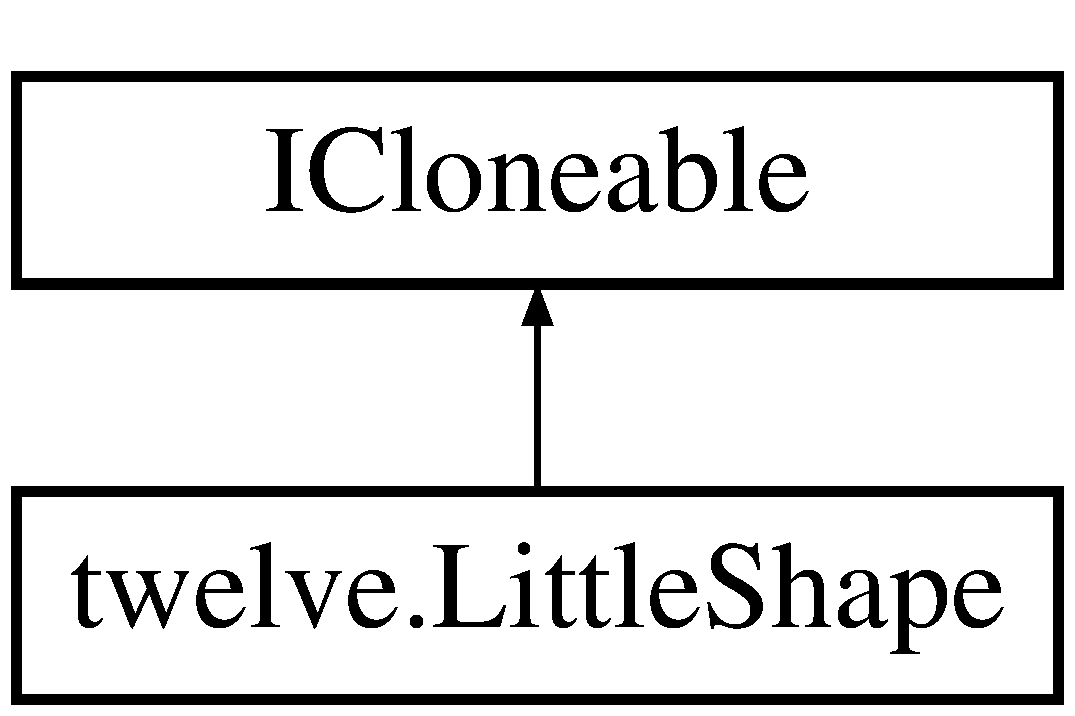
\includegraphics[height=2.000000cm]{classtwelve_1_1_little_shape}
\end{center}
\end{figure}
\subsection*{Public Member Functions}
\begin{DoxyCompactItemize}
\item 
\hypertarget{classtwelve_1_1_little_shape_aac507ba1a6214fce9a2857804fafabcf}{}void {\bfseries add} (Line l)\label{classtwelve_1_1_little_shape_aac507ba1a6214fce9a2857804fafabcf}

\item 
Line \hyperlink{classtwelve_1_1_little_shape_a824f2bd97f3ddd24731c469d23d03231}{get\+Next} ()
\begin{DoxyCompactList}\small\item\em выдает следущюю линию \end{DoxyCompactList}\item 
Point\+F\mbox{[}$\,$\mbox{]} \hyperlink{classtwelve_1_1_little_shape_acbc95b796f87111791079e7251bf204c}{get\+Point\+F} ()
\begin{DoxyCompactList}\small\item\em все точки в линии в упорядочненом массиве \end{DoxyCompactList}\item 
void \hyperlink{classtwelve_1_1_little_shape_aaa59136e3578ebf787caf75f8b1c46e9}{set\+Point\+F} (Point\+F\mbox{[}$\,$\mbox{]} p)
\begin{DoxyCompactList}\small\item\em назад в линию после трансформации \end{DoxyCompactList}\item 
\hypertarget{classtwelve_1_1_little_shape_a4a8f5f965efe82ee86b31fe9ded181d9}{}{\bfseries Little\+Shape} (\hyperlink{classtwelve_1_1_little_shape}{Little\+Shape} obj)\label{classtwelve_1_1_little_shape_a4a8f5f965efe82ee86b31fe9ded181d9}

\item 
\hypertarget{classtwelve_1_1_little_shape_a54b1df32bdb8908653e9af3142ed61c3}{}object {\bfseries Clone} ()\label{classtwelve_1_1_little_shape_a54b1df32bdb8908653e9af3142ed61c3}

\end{DoxyCompactItemize}
\subsection*{Public Attributes}
\begin{DoxyCompactItemize}
\item 
\hypertarget{classtwelve_1_1_little_shape_abcb8b597f398eaf6dbe113d10ca80766}{}List$<$ Line $>$ {\bfseries path} = new List$<$Line$>$()\label{classtwelve_1_1_little_shape_abcb8b597f398eaf6dbe113d10ca80766}

\item 
\hypertarget{classtwelve_1_1_little_shape_ad10698b2c298037d01c34b20d566d296}{}List$<$ double $>$ {\bfseries path2} = new List$<$double$>$()\label{classtwelve_1_1_little_shape_ad10698b2c298037d01c34b20d566d296}

\end{DoxyCompactItemize}
\subsection*{Properties}
\begin{DoxyCompactItemize}
\item 
\hypertarget{classtwelve_1_1_little_shape_adcfc76a7f81c1f037b44575ce2ff7cdb}{}int {\bfseries Mass}\hspace{0.3cm}{\ttfamily  \mbox{[}get, set\mbox{]}}\label{classtwelve_1_1_little_shape_adcfc76a7f81c1f037b44575ce2ff7cdb}

\end{DoxyCompactItemize}


\subsection{Detailed Description}
инкаплсулирует ломаную линию 



\subsection{Member Function Documentation}
\hypertarget{classtwelve_1_1_little_shape_a824f2bd97f3ddd24731c469d23d03231}{}\index{twelve\+::\+Little\+Shape@{twelve\+::\+Little\+Shape}!get\+Next@{get\+Next}}
\index{get\+Next@{get\+Next}!twelve\+::\+Little\+Shape@{twelve\+::\+Little\+Shape}}
\subsubsection[{get\+Next}]{\setlength{\rightskip}{0pt plus 5cm}Line twelve.\+Little\+Shape.\+get\+Next (
\begin{DoxyParamCaption}
{}
\end{DoxyParamCaption}
)}\label{classtwelve_1_1_little_shape_a824f2bd97f3ddd24731c469d23d03231}


выдает следущюю линию 

\begin{DoxyReturn}{Returns}
пока не N\+U\+L\+L можно брать линии
\end{DoxyReturn}
\hypertarget{classtwelve_1_1_little_shape_acbc95b796f87111791079e7251bf204c}{}\index{twelve\+::\+Little\+Shape@{twelve\+::\+Little\+Shape}!get\+Point\+F@{get\+Point\+F}}
\index{get\+Point\+F@{get\+Point\+F}!twelve\+::\+Little\+Shape@{twelve\+::\+Little\+Shape}}
\subsubsection[{get\+Point\+F}]{\setlength{\rightskip}{0pt plus 5cm}Point\+F \mbox{[}$\,$\mbox{]} twelve.\+Little\+Shape.\+get\+Point\+F (
\begin{DoxyParamCaption}
{}
\end{DoxyParamCaption}
)}\label{classtwelve_1_1_little_shape_acbc95b796f87111791079e7251bf204c}


все точки в линии в упорядочненом массиве 

\begin{DoxyReturn}{Returns}

\end{DoxyReturn}
\hypertarget{classtwelve_1_1_little_shape_aaa59136e3578ebf787caf75f8b1c46e9}{}\index{twelve\+::\+Little\+Shape@{twelve\+::\+Little\+Shape}!set\+Point\+F@{set\+Point\+F}}
\index{set\+Point\+F@{set\+Point\+F}!twelve\+::\+Little\+Shape@{twelve\+::\+Little\+Shape}}
\subsubsection[{set\+Point\+F}]{\setlength{\rightskip}{0pt plus 5cm}void twelve.\+Little\+Shape.\+set\+Point\+F (
\begin{DoxyParamCaption}
\item[{Point\+F\mbox{[}$\,$\mbox{]}}]{p}
\end{DoxyParamCaption}
)}\label{classtwelve_1_1_little_shape_aaa59136e3578ebf787caf75f8b1c46e9}


назад в линию после трансформации 

\begin{DoxyReturn}{Returns}

\end{DoxyReturn}


The documentation for this class was generated from the following file\+:\begin{DoxyCompactItemize}
\item 
D\+:/\+Git\+Progects/twelve/twelve/Little\+Shape.\+cs\end{DoxyCompactItemize}

\hypertarget{classtwelve_1_1_little_shape2}{}\section{twelve.\+Little\+Shape2 Class Reference}
\label{classtwelve_1_1_little_shape2}\index{twelve.\+Little\+Shape2@{twelve.\+Little\+Shape2}}
\subsection*{Public Member Functions}
\begin{DoxyCompactItemize}
\item 
\hypertarget{classtwelve_1_1_little_shape2_a132e681b0105e7701228442cb196447a}{}void {\bfseries set\+Angle\+List} (int round\+Point=5)\label{classtwelve_1_1_little_shape2_a132e681b0105e7701228442cb196447a}

\item 
\hypertarget{classtwelve_1_1_little_shape2_a5061e87020b45156047b6e735957d22c}{}double\mbox{[}$\,$\mbox{]} {\bfseries next\+Angle} (int index)\label{classtwelve_1_1_little_shape2_a5061e87020b45156047b6e735957d22c}

\item 
\hypertarget{classtwelve_1_1_little_shape2_aa52e7728ab46848d644ca276f6f53b65}{}Vector {\bfseries go\+To\+Vector} (Line l)\label{classtwelve_1_1_little_shape2_aa52e7728ab46848d644ca276f6f53b65}

\item 
\hypertarget{classtwelve_1_1_little_shape2_a109c34991d516f1d7cc176e819275516}{}void {\bfseries add} (double\mbox{[},\mbox{]} t, int rank)\label{classtwelve_1_1_little_shape2_a109c34991d516f1d7cc176e819275516}

\item 
Line \hyperlink{classtwelve_1_1_little_shape2_a4e04d0b57510f81ad69ef08e3ff80cce}{get\+Next} ()
\begin{DoxyCompactList}\small\item\em выдает следущюю линию \end{DoxyCompactList}\item 
Point\+F\mbox{[}$\,$\mbox{]} \hyperlink{classtwelve_1_1_little_shape2_a2b550148d37609328d78675f889395c1}{get\+Point\+F} (int rank)
\begin{DoxyCompactList}\small\item\em все точки в линии в упорядочненом массиве \end{DoxyCompactList}\item 
void \hyperlink{classtwelve_1_1_little_shape2_a5afd47e1b0b02f81975fdfc02ea0f030}{set\+Point\+F} (Point\+F\mbox{[}$\,$\mbox{]} p)
\begin{DoxyCompactList}\small\item\em назад в линию после трансформации здесь формируються линии и заполняется массив path \end{DoxyCompactList}\item 
void \hyperlink{classtwelve_1_1_little_shape2_a411ae955923dc349d1af3f49fbeb4819}{set\+Point} (System.\+Windows.\+Point\mbox{[}$\,$\mbox{]} p)
\begin{DoxyCompactList}\small\item\em назад в линию после трансформации здесь формируються линии и заполняется массив path \end{DoxyCompactList}\item 
\hypertarget{classtwelve_1_1_little_shape2_afb70047b35b1ad735b1fd88058369070}{}{\bfseries Little\+Shape2} (\hyperlink{classtwelve_1_1_little_shape2}{Little\+Shape2} obj)\label{classtwelve_1_1_little_shape2_afb70047b35b1ad735b1fd88058369070}

\item 
\hypertarget{classtwelve_1_1_little_shape2_a8b8616a97eb813d9c238851a7ed8836d}{}object {\bfseries Clone} ()\label{classtwelve_1_1_little_shape2_a8b8616a97eb813d9c238851a7ed8836d}

\item 
\hypertarget{classtwelve_1_1_little_shape2_aa293d0130792d100e133222f3108b5dd}{}{\bfseries Little\+Shape2} (int rank)\label{classtwelve_1_1_little_shape2_aa293d0130792d100e133222f3108b5dd}

\item 
\hypertarget{classtwelve_1_1_little_shape2_a14ef91d221550e2ab454e013b9dc9b78}{}List$<$ Line $>$ {\bfseries Little\+Shape2\+To\+Line} ()\label{classtwelve_1_1_little_shape2_a14ef91d221550e2ab454e013b9dc9b78}

\end{DoxyCompactItemize}
\subsection*{Public Attributes}
\begin{DoxyCompactItemize}
\item 
\hypertarget{classtwelve_1_1_little_shape2_a8639f275e5ecbb476a8f0a879f5e03f2}{}List$<$ Line $>$ {\bfseries path} = new List$<$Line$>$()\label{classtwelve_1_1_little_shape2_a8639f275e5ecbb476a8f0a879f5e03f2}

\item 
\hypertarget{classtwelve_1_1_little_shape2_aa5eb7ab1efbc1b895f5f6774f86dc43d}{}double\mbox{[}$\,$\mbox{]} {\bfseries angles\+Arr} = null\label{classtwelve_1_1_little_shape2_aa5eb7ab1efbc1b895f5f6774f86dc43d}

\end{DoxyCompactItemize}
\subsection*{Properties}
\begin{DoxyCompactItemize}
\item 
\hypertarget{classtwelve_1_1_little_shape2_a79caaef5888853a93e39ed6842209fcf}{}int {\bfseries Mass}\hspace{0.3cm}{\ttfamily  \mbox{[}get, set\mbox{]}}\label{classtwelve_1_1_little_shape2_a79caaef5888853a93e39ed6842209fcf}

\end{DoxyCompactItemize}


\subsection{Member Function Documentation}
\hypertarget{classtwelve_1_1_little_shape2_a4e04d0b57510f81ad69ef08e3ff80cce}{}\index{twelve\+::\+Little\+Shape2@{twelve\+::\+Little\+Shape2}!get\+Next@{get\+Next}}
\index{get\+Next@{get\+Next}!twelve\+::\+Little\+Shape2@{twelve\+::\+Little\+Shape2}}
\subsubsection[{get\+Next}]{\setlength{\rightskip}{0pt plus 5cm}Line twelve.\+Little\+Shape2.\+get\+Next (
\begin{DoxyParamCaption}
{}
\end{DoxyParamCaption}
)}\label{classtwelve_1_1_little_shape2_a4e04d0b57510f81ad69ef08e3ff80cce}


выдает следущюю линию 

\begin{DoxyReturn}{Returns}
пока не N\+U\+L\+L можно брать линии
\end{DoxyReturn}
\hypertarget{classtwelve_1_1_little_shape2_a2b550148d37609328d78675f889395c1}{}\index{twelve\+::\+Little\+Shape2@{twelve\+::\+Little\+Shape2}!get\+Point\+F@{get\+Point\+F}}
\index{get\+Point\+F@{get\+Point\+F}!twelve\+::\+Little\+Shape2@{twelve\+::\+Little\+Shape2}}
\subsubsection[{get\+Point\+F}]{\setlength{\rightskip}{0pt plus 5cm}Point\+F \mbox{[}$\,$\mbox{]} twelve.\+Little\+Shape2.\+get\+Point\+F (
\begin{DoxyParamCaption}
\item[{int}]{rank}
\end{DoxyParamCaption}
)}\label{classtwelve_1_1_little_shape2_a2b550148d37609328d78675f889395c1}


все точки в линии в упорядочненом массиве 

\begin{DoxyReturn}{Returns}

\end{DoxyReturn}
\hypertarget{classtwelve_1_1_little_shape2_a411ae955923dc349d1af3f49fbeb4819}{}\index{twelve\+::\+Little\+Shape2@{twelve\+::\+Little\+Shape2}!set\+Point@{set\+Point}}
\index{set\+Point@{set\+Point}!twelve\+::\+Little\+Shape2@{twelve\+::\+Little\+Shape2}}
\subsubsection[{set\+Point}]{\setlength{\rightskip}{0pt plus 5cm}void twelve.\+Little\+Shape2.\+set\+Point (
\begin{DoxyParamCaption}
\item[{System.\+Windows.\+Point\mbox{[}$\,$\mbox{]}}]{p}
\end{DoxyParamCaption}
)}\label{classtwelve_1_1_little_shape2_a411ae955923dc349d1af3f49fbeb4819}


назад в линию после трансформации здесь формируються линии и заполняется массив path 

\begin{DoxyReturn}{Returns}

\end{DoxyReturn}
\hypertarget{classtwelve_1_1_little_shape2_a5afd47e1b0b02f81975fdfc02ea0f030}{}\index{twelve\+::\+Little\+Shape2@{twelve\+::\+Little\+Shape2}!set\+Point\+F@{set\+Point\+F}}
\index{set\+Point\+F@{set\+Point\+F}!twelve\+::\+Little\+Shape2@{twelve\+::\+Little\+Shape2}}
\subsubsection[{set\+Point\+F}]{\setlength{\rightskip}{0pt plus 5cm}void twelve.\+Little\+Shape2.\+set\+Point\+F (
\begin{DoxyParamCaption}
\item[{Point\+F\mbox{[}$\,$\mbox{]}}]{p}
\end{DoxyParamCaption}
)}\label{classtwelve_1_1_little_shape2_a5afd47e1b0b02f81975fdfc02ea0f030}


назад в линию после трансформации здесь формируються линии и заполняется массив path 

\begin{DoxyReturn}{Returns}

\end{DoxyReturn}


The documentation for this class was generated from the following file\+:\begin{DoxyCompactItemize}
\item 
D\+:/\+Git\+Progects/twelve/twelve/Little\+Shape2.\+cs\end{DoxyCompactItemize}

\hypertarget{classtwelve_1_1_main_window}{}\section{twelve.\+Main\+Window Class Reference}
\label{classtwelve_1_1_main_window}\index{twelve.\+Main\+Window@{twelve.\+Main\+Window}}


Логика взаимодействия для Main\+Window.\+xaml  


Inheritance diagram for twelve.\+Main\+Window\+:\begin{figure}[H]
\begin{center}
\leavevmode
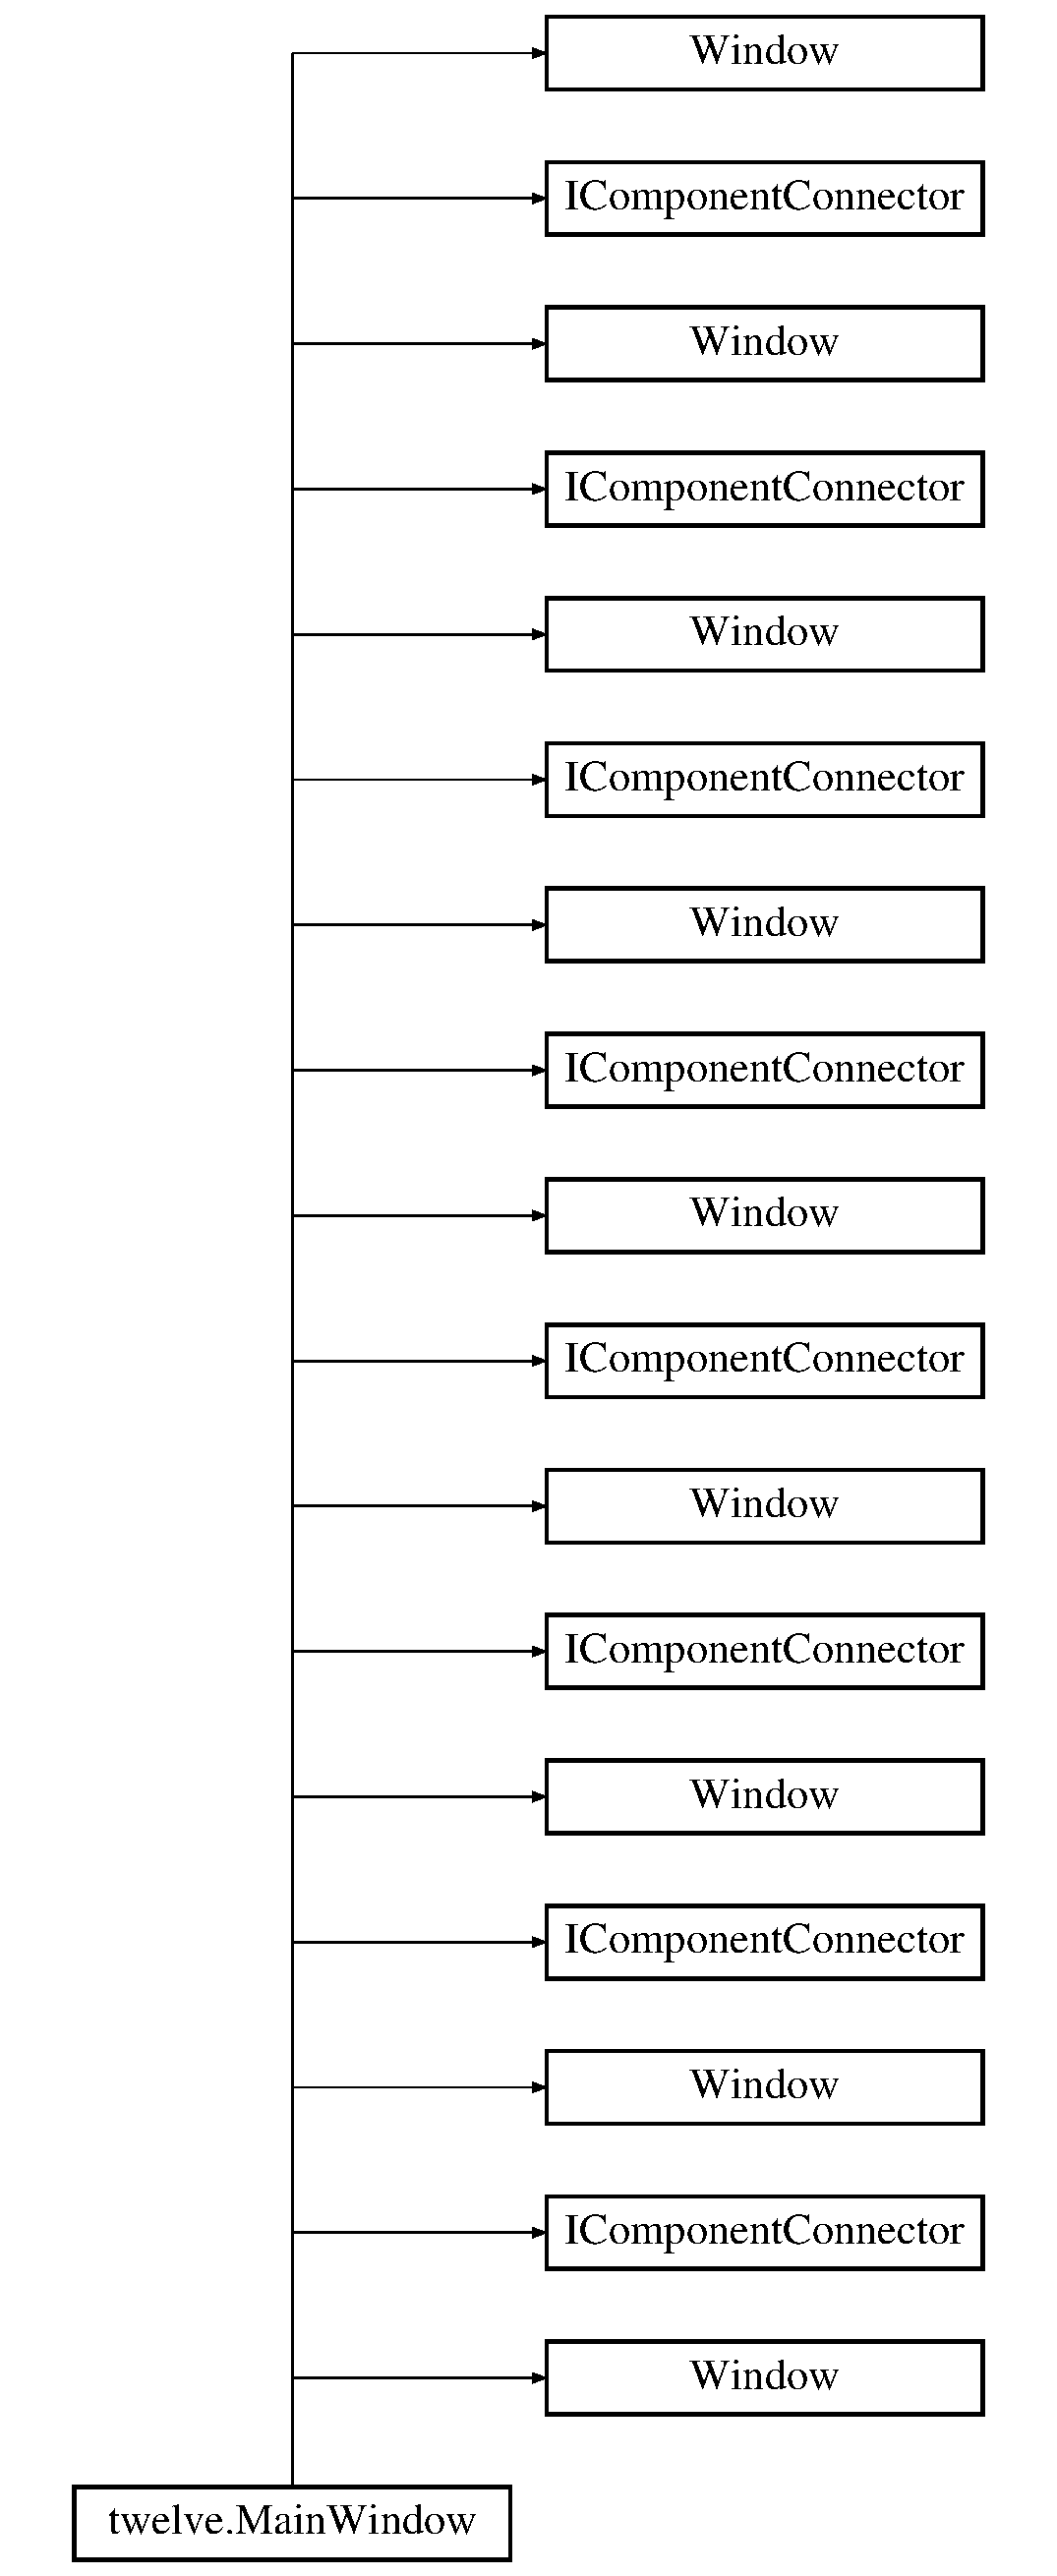
\includegraphics[height=12.000000cm]{classtwelve_1_1_main_window}
\end{center}
\end{figure}
\subsection*{Public Member Functions}
\begin{DoxyCompactItemize}
\item 
Line \hyperlink{classtwelve_1_1_main_window_a4b493a912c1d0cf8944ac182ac7a36bc}{move\+Line} (Line t, int resize\+X=350, int resize\+Y=250)
\begin{DoxyCompactList}\small\item\em смещение линии по осям \end{DoxyCompactList}\item 
void \hyperlink{classtwelve_1_1_main_window_a1bf7bff30ceb077bb52625461737dcf2}{my\+Matrix\+Transform\+Scale} (ref \hyperlink{classtwelve_1_1_little_shape2}{Little\+Shape2} temp)
\begin{DoxyCompactList}\small\item\em фун для матричного преобразования в даном случае увеличения \end{DoxyCompactList}\item 
void \hyperlink{classtwelve_1_1_main_window_a326cc47dfb711694b5cb01e9eb33db16}{my\+Matrix\+Transform\+Scale\+Mini} (ref \hyperlink{classtwelve_1_1_little_shape2}{Little\+Shape2} temp)
\begin{DoxyCompactList}\small\item\em фун для матричного преобразования в даном случае увеличения \end{DoxyCompactList}\item 
List$<$ \hyperlink{classtwelve_1_1_little_shape2}{Little\+Shape2} $>$ \hyperlink{classtwelve_1_1_main_window_aed30ff82251ce0f7896fbf22e23f406f}{selectfun} (int m)
\begin{DoxyCompactList}\small\item\em виборка всех елементов с определенной масой доделать проверку на углы \end{DoxyCompactList}\item 
\hyperlink{classtwelve_1_1_little_shape2}{Little\+Shape2} \hyperlink{classtwelve_1_1_main_window_acb1b0b5ccc4e94040a1eed2f10926f8e}{select\+One\+Shape} (int m)
\begin{DoxyCompactList}\small\item\em виборка одной фигуры по индексу \end{DoxyCompactList}\item 
\hypertarget{classtwelve_1_1_main_window_a6113105ef67052bc0b5598f02799a120}{}bool {\bfseries equal\+Arr\+Double} (double\mbox{[}$\,$\mbox{]} a, double\mbox{[}$\,$\mbox{]} b)\label{classtwelve_1_1_main_window_a6113105ef67052bc0b5598f02799a120}

\item 
\hypertarget{classtwelve_1_1_main_window_a829c67c5bd13de56ee264abf658762dc}{}void {\bfseries figure\+Info} (\hyperlink{classtwelve_1_1_little_shape2}{Little\+Shape2} temp2)\label{classtwelve_1_1_main_window_a829c67c5bd13de56ee264abf658762dc}

\item 
\hypertarget{classtwelve_1_1_main_window_a0da87738c75f6d89f0d03070474543fe}{}Canvas {\bfseries cuprent\+Picture} ()\label{classtwelve_1_1_main_window_a0da87738c75f6d89f0d03070474543fe}

\item 
void \hyperlink{classtwelve_1_1_main_window_aedcedf38ae172b730e9b86fd91b8bb75}{showin\+Console\+Debug} (String s, bool x)
\item 
Canvas \hyperlink{classtwelve_1_1_main_window_a5fe1ea86efca790d66e7c803dec7a666}{Stream\+Geometry\+Triangle\+Litle} (List$<$ System.\+Windows.\+Point $>$ arr\+Points)
\begin{DoxyCompactList}\small\item\em обработчик ТЕСТ кнопки \end{DoxyCompactList}\item 
void \hyperlink{classtwelve_1_1_main_window_a8b4ddfee953ce2787f242eaaaefaa26c}{Stream\+Geometry\+Triangle\+Example} (List$<$ System.\+Windows.\+Point $>$ arr\+Points)
\begin{DoxyCompactList}\small\item\em рисовалка для фигуры \end{DoxyCompactList}\item 
void \hyperlink{classtwelve_1_1_main_window_a3b53f5fa36890e3451372782b73b54d1}{Initialize\+Component} ()
\begin{DoxyCompactList}\small\item\em Initialize\+Component \end{DoxyCompactList}\item 
void \hyperlink{classtwelve_1_1_main_window_a3b53f5fa36890e3451372782b73b54d1}{Initialize\+Component} ()
\begin{DoxyCompactList}\small\item\em Initialize\+Component \end{DoxyCompactList}\item 
void \hyperlink{classtwelve_1_1_main_window_a3b53f5fa36890e3451372782b73b54d1}{Initialize\+Component} ()
\begin{DoxyCompactList}\small\item\em Initialize\+Component \end{DoxyCompactList}\item 
void \hyperlink{classtwelve_1_1_main_window_a3b53f5fa36890e3451372782b73b54d1}{Initialize\+Component} ()
\begin{DoxyCompactList}\small\item\em Initialize\+Component \end{DoxyCompactList}\item 
void \hyperlink{classtwelve_1_1_main_window_a3b53f5fa36890e3451372782b73b54d1}{Initialize\+Component} ()
\begin{DoxyCompactList}\small\item\em Initialize\+Component \end{DoxyCompactList}\item 
void \hyperlink{classtwelve_1_1_main_window_a3b53f5fa36890e3451372782b73b54d1}{Initialize\+Component} ()
\begin{DoxyCompactList}\small\item\em Initialize\+Component \end{DoxyCompactList}\item 
void \hyperlink{classtwelve_1_1_main_window_a3b53f5fa36890e3451372782b73b54d1}{Initialize\+Component} ()
\begin{DoxyCompactList}\small\item\em Initialize\+Component \end{DoxyCompactList}\item 
void \hyperlink{classtwelve_1_1_main_window_a3b53f5fa36890e3451372782b73b54d1}{Initialize\+Component} ()
\begin{DoxyCompactList}\small\item\em Initialize\+Component \end{DoxyCompactList}\end{DoxyCompactItemize}


\subsection{Detailed Description}
Логика взаимодействия для Main\+Window.\+xaml 

\hyperlink{classtwelve_1_1_main_window}{Main\+Window} 

\subsection{Member Function Documentation}
\hypertarget{classtwelve_1_1_main_window_a3b53f5fa36890e3451372782b73b54d1}{}\index{twelve\+::\+Main\+Window@{twelve\+::\+Main\+Window}!Initialize\+Component@{Initialize\+Component}}
\index{Initialize\+Component@{Initialize\+Component}!twelve\+::\+Main\+Window@{twelve\+::\+Main\+Window}}
\subsubsection[{Initialize\+Component}]{\setlength{\rightskip}{0pt plus 5cm}void twelve.\+Main\+Window.\+Initialize\+Component (
\begin{DoxyParamCaption}
{}
\end{DoxyParamCaption}
)}\label{classtwelve_1_1_main_window_a3b53f5fa36890e3451372782b73b54d1}


Initialize\+Component 

\hypertarget{classtwelve_1_1_main_window_a3b53f5fa36890e3451372782b73b54d1}{}\index{twelve\+::\+Main\+Window@{twelve\+::\+Main\+Window}!Initialize\+Component@{Initialize\+Component}}
\index{Initialize\+Component@{Initialize\+Component}!twelve\+::\+Main\+Window@{twelve\+::\+Main\+Window}}
\subsubsection[{Initialize\+Component}]{\setlength{\rightskip}{0pt plus 5cm}void twelve.\+Main\+Window.\+Initialize\+Component (
\begin{DoxyParamCaption}
{}
\end{DoxyParamCaption}
)}\label{classtwelve_1_1_main_window_a3b53f5fa36890e3451372782b73b54d1}


Initialize\+Component 

\hypertarget{classtwelve_1_1_main_window_a3b53f5fa36890e3451372782b73b54d1}{}\index{twelve\+::\+Main\+Window@{twelve\+::\+Main\+Window}!Initialize\+Component@{Initialize\+Component}}
\index{Initialize\+Component@{Initialize\+Component}!twelve\+::\+Main\+Window@{twelve\+::\+Main\+Window}}
\subsubsection[{Initialize\+Component}]{\setlength{\rightskip}{0pt plus 5cm}void twelve.\+Main\+Window.\+Initialize\+Component (
\begin{DoxyParamCaption}
{}
\end{DoxyParamCaption}
)}\label{classtwelve_1_1_main_window_a3b53f5fa36890e3451372782b73b54d1}


Initialize\+Component 

\hypertarget{classtwelve_1_1_main_window_a3b53f5fa36890e3451372782b73b54d1}{}\index{twelve\+::\+Main\+Window@{twelve\+::\+Main\+Window}!Initialize\+Component@{Initialize\+Component}}
\index{Initialize\+Component@{Initialize\+Component}!twelve\+::\+Main\+Window@{twelve\+::\+Main\+Window}}
\subsubsection[{Initialize\+Component}]{\setlength{\rightskip}{0pt plus 5cm}void twelve.\+Main\+Window.\+Initialize\+Component (
\begin{DoxyParamCaption}
{}
\end{DoxyParamCaption}
)}\label{classtwelve_1_1_main_window_a3b53f5fa36890e3451372782b73b54d1}


Initialize\+Component 

\hypertarget{classtwelve_1_1_main_window_a3b53f5fa36890e3451372782b73b54d1}{}\index{twelve\+::\+Main\+Window@{twelve\+::\+Main\+Window}!Initialize\+Component@{Initialize\+Component}}
\index{Initialize\+Component@{Initialize\+Component}!twelve\+::\+Main\+Window@{twelve\+::\+Main\+Window}}
\subsubsection[{Initialize\+Component}]{\setlength{\rightskip}{0pt plus 5cm}void twelve.\+Main\+Window.\+Initialize\+Component (
\begin{DoxyParamCaption}
{}
\end{DoxyParamCaption}
)}\label{classtwelve_1_1_main_window_a3b53f5fa36890e3451372782b73b54d1}


Initialize\+Component 

\hypertarget{classtwelve_1_1_main_window_a3b53f5fa36890e3451372782b73b54d1}{}\index{twelve\+::\+Main\+Window@{twelve\+::\+Main\+Window}!Initialize\+Component@{Initialize\+Component}}
\index{Initialize\+Component@{Initialize\+Component}!twelve\+::\+Main\+Window@{twelve\+::\+Main\+Window}}
\subsubsection[{Initialize\+Component}]{\setlength{\rightskip}{0pt plus 5cm}void twelve.\+Main\+Window.\+Initialize\+Component (
\begin{DoxyParamCaption}
{}
\end{DoxyParamCaption}
)}\label{classtwelve_1_1_main_window_a3b53f5fa36890e3451372782b73b54d1}


Initialize\+Component 

\hypertarget{classtwelve_1_1_main_window_a3b53f5fa36890e3451372782b73b54d1}{}\index{twelve\+::\+Main\+Window@{twelve\+::\+Main\+Window}!Initialize\+Component@{Initialize\+Component}}
\index{Initialize\+Component@{Initialize\+Component}!twelve\+::\+Main\+Window@{twelve\+::\+Main\+Window}}
\subsubsection[{Initialize\+Component}]{\setlength{\rightskip}{0pt plus 5cm}void twelve.\+Main\+Window.\+Initialize\+Component (
\begin{DoxyParamCaption}
{}
\end{DoxyParamCaption}
)}\label{classtwelve_1_1_main_window_a3b53f5fa36890e3451372782b73b54d1}


Initialize\+Component 

\hypertarget{classtwelve_1_1_main_window_a3b53f5fa36890e3451372782b73b54d1}{}\index{twelve\+::\+Main\+Window@{twelve\+::\+Main\+Window}!Initialize\+Component@{Initialize\+Component}}
\index{Initialize\+Component@{Initialize\+Component}!twelve\+::\+Main\+Window@{twelve\+::\+Main\+Window}}
\subsubsection[{Initialize\+Component}]{\setlength{\rightskip}{0pt plus 5cm}void twelve.\+Main\+Window.\+Initialize\+Component (
\begin{DoxyParamCaption}
{}
\end{DoxyParamCaption}
)}\label{classtwelve_1_1_main_window_a3b53f5fa36890e3451372782b73b54d1}


Initialize\+Component 

\hypertarget{classtwelve_1_1_main_window_a4b493a912c1d0cf8944ac182ac7a36bc}{}\index{twelve\+::\+Main\+Window@{twelve\+::\+Main\+Window}!move\+Line@{move\+Line}}
\index{move\+Line@{move\+Line}!twelve\+::\+Main\+Window@{twelve\+::\+Main\+Window}}
\subsubsection[{move\+Line}]{\setlength{\rightskip}{0pt plus 5cm}Line twelve.\+Main\+Window.\+move\+Line (
\begin{DoxyParamCaption}
\item[{Line}]{t, }
\item[{int}]{resize\+X = {\ttfamily 350}, }
\item[{int}]{resize\+Y = {\ttfamily 250}}
\end{DoxyParamCaption}
)}\label{classtwelve_1_1_main_window_a4b493a912c1d0cf8944ac182ac7a36bc}


смещение линии по осям 


\begin{DoxyParams}{Parameters}
{\em line} & передача по ссилке\\
\hline
{\em y} & \\
\hline
\end{DoxyParams}
/// 
\begin{DoxyParams}{Parameters}
{\em y} & \\
\hline
\end{DoxyParams}
\begin{DoxyReturn}{Returns}

\end{DoxyReturn}
\hypertarget{classtwelve_1_1_main_window_a1bf7bff30ceb077bb52625461737dcf2}{}\index{twelve\+::\+Main\+Window@{twelve\+::\+Main\+Window}!my\+Matrix\+Transform\+Scale@{my\+Matrix\+Transform\+Scale}}
\index{my\+Matrix\+Transform\+Scale@{my\+Matrix\+Transform\+Scale}!twelve\+::\+Main\+Window@{twelve\+::\+Main\+Window}}
\subsubsection[{my\+Matrix\+Transform\+Scale}]{\setlength{\rightskip}{0pt plus 5cm}void twelve.\+Main\+Window.\+my\+Matrix\+Transform\+Scale (
\begin{DoxyParamCaption}
\item[{ref {\bf Little\+Shape2}}]{temp}
\end{DoxyParamCaption}
)}\label{classtwelve_1_1_main_window_a1bf7bff30ceb077bb52625461737dcf2}


фун для матричного преобразования в даном случае увеличения 


\begin{DoxyParams}{Parameters}
{\em temp} & \\
\hline
\end{DoxyParams}
\hypertarget{classtwelve_1_1_main_window_a326cc47dfb711694b5cb01e9eb33db16}{}\index{twelve\+::\+Main\+Window@{twelve\+::\+Main\+Window}!my\+Matrix\+Transform\+Scale\+Mini@{my\+Matrix\+Transform\+Scale\+Mini}}
\index{my\+Matrix\+Transform\+Scale\+Mini@{my\+Matrix\+Transform\+Scale\+Mini}!twelve\+::\+Main\+Window@{twelve\+::\+Main\+Window}}
\subsubsection[{my\+Matrix\+Transform\+Scale\+Mini}]{\setlength{\rightskip}{0pt plus 5cm}void twelve.\+Main\+Window.\+my\+Matrix\+Transform\+Scale\+Mini (
\begin{DoxyParamCaption}
\item[{ref {\bf Little\+Shape2}}]{temp}
\end{DoxyParamCaption}
)}\label{classtwelve_1_1_main_window_a326cc47dfb711694b5cb01e9eb33db16}


фун для матричного преобразования в даном случае увеличения 


\begin{DoxyParams}{Parameters}
{\em temp} & \\
\hline
\end{DoxyParams}
\hypertarget{classtwelve_1_1_main_window_aed30ff82251ce0f7896fbf22e23f406f}{}\index{twelve\+::\+Main\+Window@{twelve\+::\+Main\+Window}!selectfun@{selectfun}}
\index{selectfun@{selectfun}!twelve\+::\+Main\+Window@{twelve\+::\+Main\+Window}}
\subsubsection[{selectfun}]{\setlength{\rightskip}{0pt plus 5cm}List$<${\bf Little\+Shape2}$>$ twelve.\+Main\+Window.\+selectfun (
\begin{DoxyParamCaption}
\item[{int}]{m}
\end{DoxyParamCaption}
)}\label{classtwelve_1_1_main_window_aed30ff82251ce0f7896fbf22e23f406f}


виборка всех елементов с определенной масой доделать проверку на углы 


\begin{DoxyParams}{Parameters}
{\em mass} & \\
\hline
\end{DoxyParams}
\hypertarget{classtwelve_1_1_main_window_acb1b0b5ccc4e94040a1eed2f10926f8e}{}\index{twelve\+::\+Main\+Window@{twelve\+::\+Main\+Window}!select\+One\+Shape@{select\+One\+Shape}}
\index{select\+One\+Shape@{select\+One\+Shape}!twelve\+::\+Main\+Window@{twelve\+::\+Main\+Window}}
\subsubsection[{select\+One\+Shape}]{\setlength{\rightskip}{0pt plus 5cm}{\bf Little\+Shape2} twelve.\+Main\+Window.\+select\+One\+Shape (
\begin{DoxyParamCaption}
\item[{int}]{m}
\end{DoxyParamCaption}
)}\label{classtwelve_1_1_main_window_acb1b0b5ccc4e94040a1eed2f10926f8e}


виборка одной фигуры по индексу 


\begin{DoxyParams}{Parameters}
{\em mass} & \\
\hline
\end{DoxyParams}
\hypertarget{classtwelve_1_1_main_window_aedcedf38ae172b730e9b86fd91b8bb75}{}\index{twelve\+::\+Main\+Window@{twelve\+::\+Main\+Window}!showin\+Console\+Debug@{showin\+Console\+Debug}}
\index{showin\+Console\+Debug@{showin\+Console\+Debug}!twelve\+::\+Main\+Window@{twelve\+::\+Main\+Window}}
\subsubsection[{showin\+Console\+Debug}]{\setlength{\rightskip}{0pt plus 5cm}void twelve.\+Main\+Window.\+showin\+Console\+Debug (
\begin{DoxyParamCaption}
\item[{String}]{s, }
\item[{bool}]{x}
\end{DoxyParamCaption}
)}\label{classtwelve_1_1_main_window_aedcedf38ae172b730e9b86fd91b8bb75}




вывод или в консоль + или в документ пока textik 


\begin{DoxyParams}{Parameters}
{\em s} & \\
\hline
{\em x} & \\
\hline
\end{DoxyParams}
\hypertarget{classtwelve_1_1_main_window_a8b4ddfee953ce2787f242eaaaefaa26c}{}\index{twelve\+::\+Main\+Window@{twelve\+::\+Main\+Window}!Stream\+Geometry\+Triangle\+Example@{Stream\+Geometry\+Triangle\+Example}}
\index{Stream\+Geometry\+Triangle\+Example@{Stream\+Geometry\+Triangle\+Example}!twelve\+::\+Main\+Window@{twelve\+::\+Main\+Window}}
\subsubsection[{Stream\+Geometry\+Triangle\+Example}]{\setlength{\rightskip}{0pt plus 5cm}void twelve.\+Main\+Window.\+Stream\+Geometry\+Triangle\+Example (
\begin{DoxyParamCaption}
\item[{List$<$ System.\+Windows.\+Point $>$}]{arr\+Points}
\end{DoxyParamCaption}
)}\label{classtwelve_1_1_main_window_a8b4ddfee953ce2787f242eaaaefaa26c}


рисовалка для фигуры 


\begin{DoxyParams}{Parameters}
{\em arr\+Points} & \\
\hline
\end{DoxyParams}
\hypertarget{classtwelve_1_1_main_window_a5fe1ea86efca790d66e7c803dec7a666}{}\index{twelve\+::\+Main\+Window@{twelve\+::\+Main\+Window}!Stream\+Geometry\+Triangle\+Litle@{Stream\+Geometry\+Triangle\+Litle}}
\index{Stream\+Geometry\+Triangle\+Litle@{Stream\+Geometry\+Triangle\+Litle}!twelve\+::\+Main\+Window@{twelve\+::\+Main\+Window}}
\subsubsection[{Stream\+Geometry\+Triangle\+Litle}]{\setlength{\rightskip}{0pt plus 5cm}Canvas twelve.\+Main\+Window.\+Stream\+Geometry\+Triangle\+Litle (
\begin{DoxyParamCaption}
\item[{List$<$ System.\+Windows.\+Point $>$}]{arr\+Points}
\end{DoxyParamCaption}
)}\label{classtwelve_1_1_main_window_a5fe1ea86efca790d66e7c803dec7a666}


обработчик ТЕСТ кнопки 


\begin{DoxyParams}{Parameters}
{\em sender} & \\
\hline
{\em e} & \\
\hline
\end{DoxyParams}


рисовалка для фигуры 


\begin{DoxyParams}{Parameters}
{\em arr\+Points} & \\
\hline
\end{DoxyParams}


The documentation for this class was generated from the following files\+:\begin{DoxyCompactItemize}
\item 
D\+:/\+Git\+Progects/twelve/twelve/Main\+Window.\+xaml.\+cs\item 
D\+:/\+Git\+Progects/twelve/twelve/obj/\+Debug/Main\+Window.\+g.\+cs\item 
D\+:/\+Git\+Progects/twelve/twelve/obj/\+Debug/Main\+Window.\+g.\+i.\+cs\end{DoxyCompactItemize}

\hypertarget{classtwelve_1_1_my_data_grid_item}{}\section{twelve.\+My\+Data\+Grid\+Item Class Reference}
\label{classtwelve_1_1_my_data_grid_item}\index{twelve.\+My\+Data\+Grid\+Item@{twelve.\+My\+Data\+Grid\+Item}}
\subsection*{Properties}
\begin{DoxyCompactItemize}
\item 
\hypertarget{classtwelve_1_1_my_data_grid_item_ab81c03c19d638f1069228fefc718ef09}{}Canvas {\bfseries Image}\hspace{0.3cm}{\ttfamily  \mbox{[}get, set\mbox{]}}\label{classtwelve_1_1_my_data_grid_item_ab81c03c19d638f1069228fefc718ef09}

\item 
\hypertarget{classtwelve_1_1_my_data_grid_item_a42b788fffd89b383429f1f60f67e1045}{}string {\bfseries Description}\hspace{0.3cm}{\ttfamily  \mbox{[}get, set\mbox{]}}\label{classtwelve_1_1_my_data_grid_item_a42b788fffd89b383429f1f60f67e1045}

\end{DoxyCompactItemize}


The documentation for this class was generated from the following file\+:\begin{DoxyCompactItemize}
\item 
D\+:/\+Git\+Progects/twelve/twelve/My\+Data\+Grid\+Item.\+cs\end{DoxyCompactItemize}

\hypertarget{classtwelve_1_1_my_matrix}{}\section{twelve.\+My\+Matrix Class Reference}
\label{classtwelve_1_1_my_matrix}\index{twelve.\+My\+Matrix@{twelve.\+My\+Matrix}}
\subsection*{Public Member Functions}
\begin{DoxyCompactItemize}
\item 
\hypertarget{classtwelve_1_1_my_matrix_a1b3ed177c9205adf7a87748f5f004507}{}{\bfseries My\+Matrix} (float\mbox{[}$\,$\mbox{]} a1, float\mbox{[}$\,$\mbox{]} a2, float\mbox{[}$\,$\mbox{]} a3)\label{classtwelve_1_1_my_matrix_a1b3ed177c9205adf7a87748f5f004507}

\item 
Point\+F \hyperlink{classtwelve_1_1_my_matrix_a849cca65bed6d7bfcdc05b116ac8e6cf}{multy1} (float\mbox{[}$\,$\mbox{]} a\+N)
\begin{DoxyCompactList}\small\item\em матричное умножение \end{DoxyCompactList}\end{DoxyCompactItemize}


\subsection{Member Function Documentation}
\hypertarget{classtwelve_1_1_my_matrix_a849cca65bed6d7bfcdc05b116ac8e6cf}{}\index{twelve\+::\+My\+Matrix@{twelve\+::\+My\+Matrix}!multy1@{multy1}}
\index{multy1@{multy1}!twelve\+::\+My\+Matrix@{twelve\+::\+My\+Matrix}}
\subsubsection[{multy1}]{\setlength{\rightskip}{0pt plus 5cm}Point\+F twelve.\+My\+Matrix.\+multy1 (
\begin{DoxyParamCaption}
\item[{float\mbox{[}$\,$\mbox{]}}]{a\+N}
\end{DoxyParamCaption}
)}\label{classtwelve_1_1_my_matrix_a849cca65bed6d7bfcdc05b116ac8e6cf}


матричное умножение 


\begin{DoxyParams}{Parameters}
{\em a} & x,y,z точки\\
\hline
\end{DoxyParams}


The documentation for this class was generated from the following file\+:\begin{DoxyCompactItemize}
\item 
D\+:/\+Git\+Progects/twelve/twelve/My\+Matrix.\+cs\end{DoxyCompactItemize}

\hypertarget{classtwelve_1_1_painter}{}\section{twelve.\+Painter Class Reference}
\label{classtwelve_1_1_painter}\index{twelve.\+Painter@{twelve.\+Painter}}


класс для рисования фигур  


\subsection*{Public Member Functions}
\begin{DoxyCompactItemize}
\item 
\hyperlink{classtwelve_1_1_painter_ac255c01832d4193a56ae7970ce5f89cb}{Painter} (List$<$ Point\+Collection $>$ p)
\begin{DoxyCompactList}\small\item\em конструктор \end{DoxyCompactList}\item 
Point\+Collection \hyperlink{classtwelve_1_1_painter_a78b40befdad73558084ce99fee95d949}{get\+Next} ()
\begin{DoxyCompactList}\small\item\em возврат следцющей фигуры для рисования \end{DoxyCompactList}\item 
Point\+Collection \hyperlink{classtwelve_1_1_painter_aad43b013c8b8feef706816916c6c18ff}{get\+Prev} ()
\begin{DoxyCompactList}\small\item\em возврат предыдцщей фигуры для рисования \end{DoxyCompactList}\end{DoxyCompactItemize}


\subsection{Detailed Description}
класс для рисования фигур 



\subsection{Constructor \& Destructor Documentation}
\hypertarget{classtwelve_1_1_painter_ac255c01832d4193a56ae7970ce5f89cb}{}\index{twelve\+::\+Painter@{twelve\+::\+Painter}!Painter@{Painter}}
\index{Painter@{Painter}!twelve\+::\+Painter@{twelve\+::\+Painter}}
\subsubsection[{Painter}]{\setlength{\rightskip}{0pt plus 5cm}twelve.\+Painter.\+Painter (
\begin{DoxyParamCaption}
\item[{List$<$ Point\+Collection $>$}]{p}
\end{DoxyParamCaption}
)}\label{classtwelve_1_1_painter_ac255c01832d4193a56ae7970ce5f89cb}


конструктор 


\begin{DoxyParams}{Parameters}
{\em p} & все фигуры с определеной площадю\\
\hline
\end{DoxyParams}


\subsection{Member Function Documentation}
\hypertarget{classtwelve_1_1_painter_a78b40befdad73558084ce99fee95d949}{}\index{twelve\+::\+Painter@{twelve\+::\+Painter}!get\+Next@{get\+Next}}
\index{get\+Next@{get\+Next}!twelve\+::\+Painter@{twelve\+::\+Painter}}
\subsubsection[{get\+Next}]{\setlength{\rightskip}{0pt plus 5cm}Point\+Collection twelve.\+Painter.\+get\+Next (
\begin{DoxyParamCaption}
{}
\end{DoxyParamCaption}
)}\label{classtwelve_1_1_painter_a78b40befdad73558084ce99fee95d949}


возврат следцющей фигуры для рисования 

\begin{DoxyReturn}{Returns}
Path
\end{DoxyReturn}
\hypertarget{classtwelve_1_1_painter_aad43b013c8b8feef706816916c6c18ff}{}\index{twelve\+::\+Painter@{twelve\+::\+Painter}!get\+Prev@{get\+Prev}}
\index{get\+Prev@{get\+Prev}!twelve\+::\+Painter@{twelve\+::\+Painter}}
\subsubsection[{get\+Prev}]{\setlength{\rightskip}{0pt plus 5cm}Point\+Collection twelve.\+Painter.\+get\+Prev (
\begin{DoxyParamCaption}
{}
\end{DoxyParamCaption}
)}\label{classtwelve_1_1_painter_aad43b013c8b8feef706816916c6c18ff}


возврат предыдцщей фигуры для рисования 

\begin{DoxyReturn}{Returns}
Path 
\end{DoxyReturn}


The documentation for this class was generated from the following file\+:\begin{DoxyCompactItemize}
\item 
D\+:/\+Git\+Progects/twelve/twelve/Painter.\+cs\end{DoxyCompactItemize}

\hypertarget{classtesstthread_1_1_program}{}\section{tesstthread.\+Program Class Reference}
\label{classtesstthread_1_1_program}\index{tesstthread.\+Program@{tesstthread.\+Program}}


The documentation for this class was generated from the following file\+:\begin{DoxyCompactItemize}
\item 
D\+:/\+Git\+Progects/twelve/tesstthread/Program.\+cs\end{DoxyCompactItemize}

\hypertarget{classtwelve_1_1_tester}{}\section{twelve.\+Tester Class Reference}
\label{classtwelve_1_1_tester}\index{twelve.\+Tester@{twelve.\+Tester}}
\subsection*{Public Member Functions}
\begin{DoxyCompactItemize}
\item 
\hypertarget{classtwelve_1_1_tester_adb766d6122378b679b3d5a9dcf882789}{}void {\bfseries draw} (Canvas canvas)\label{classtwelve_1_1_tester_adb766d6122378b679b3d5a9dcf882789}

\item 
\hypertarget{classtwelve_1_1_tester_aca4ac437d1e133e5d1bbff31860ae0a5}{}void {\bfseries Render\+Target\+Bitmap\+Example} ()\label{classtwelve_1_1_tester_aca4ac437d1e133e5d1bbff31860ae0a5}

\end{DoxyCompactItemize}


The documentation for this class was generated from the following file\+:\begin{DoxyCompactItemize}
\item 
D\+:/\+Git\+Progects/twelve/twelve/Tester.\+cs\end{DoxyCompactItemize}

%--- End generated contents ---

% Index
\backmatter
\newpage
\phantomsection
\clearemptydoublepage
\addcontentsline{toc}{chapter}{Index}
\printindex

\end{document}
